%%% Version 2.5 Generated 2022/06/14 %%%
%%% You will need to have the following packages installed: datetime, fmtcount, etoolbox, fcprefix, which are normally inlcuded in WinEdt. %%%
%%% In http://www.ctan.org/ you can find the packages and how to install them, if necessary. %%%
%%%  NB logo1.jpg is required in the path in order to correctly compile front page header %%%

\documentclass[utf8]{frontiers_suppmat} % for all articles
\usepackage{url,hyperref,lineno,microtype,booktabs}
\usepackage[onehalfspacing]{setspace}
\usepackage{float} % Added to force float placement



% Leave a blank line between paragraphs instead of using \\

\begin{document}
\graphicspath{{paper_figures/}}

\onecolumn
\firstpage{1}

\title[Supplementary Material]{{\helveticaitalic{Supplementary Material}}}


\maketitle

\section{Falsification Protocol Controls}
\label{sec:supp-falsification}

\subsection{Controls, by claim.}

\begin{itemize}
  \item \textbf{C1 : round-0 baseline.} Cluster quality computed before any
    federated training. If already high, pretrained representations are
    doing the work, not federated learning.
  \item \textbf{C2 : isolated local training.} Each silo trains
    independently, with no aggregation step at all. If isolated training
    reaches the same cluster-quality trajectory as federated training,
    federation's contribution to representation quality specifically is not
    demonstrated, regardless of whether training in general works.
  \item \textbf{C3 : shuffled-label control.} Training proceeds with
    disease labels randomly permuted across examples (text unchanged,
    text:label correspondence broken). If disease clusters still form when
    evaluated against the \emph{true} labels, the signal is driven by
    surface text features rather than learned disease identity, and is
    spurious.
  \item \textbf{C4 : known-disease control injection.} A disease the model
    already knows is injected mid-simulation under a fake ``unknown'' label,
    using the identical mechanism, timing, and seed offset as a genuine novel-
    disease injection. A trustworthy detector should absorb these examples
    into the disease's existing cluster rather than reporting a new one;
    if it instead reports a confident new cluster, the evaluation method
    itself is unreliable, independent of whether genuine novel-disease
    detection elsewhere looks correct.
  \item \textbf{C5 : untrained held-out-class absorption control.} Tests
    whether the \texttt{PrototypeBank}'s ``unknown'' bucket absorbs content
    that is genuinely novel but completely unrelated to the target disease
    --- i.e., an OOD class the model never trained on. If any novel-looking
    embedding lands in the unknown cluster, it gets flagged as a candidate
    novel disease even if it has nothing to do with the injected pathogen.
\end{itemize}

\subsection{Decision rule.} A control that passes does not, on its own,
establish either claim; a control that fails identifies a specific,
nameable alternative explanation that must be addressed (by a methodological
fix, such as a different evaluation procedure, or by a narrowed claim) before
the corresponding result can be reported without qualification.


\section{System Prompts}
\label{sec:supp-system-prompts}

All three LLM roles receive system prompts generated at runtime by
\texttt{simulation.fictional\_diseases}. The disease-knowledge block
(definitions, key symptoms, characteristic vitals) is identical across
the nurse and doctor roles; role-specific instructions determine the
permitted response types and output format. The patient prompt is
parameterised by the patient's assigned disease.

\subsection{Nurse prompt}

{\footnotesize
\begin{verbatim}
You are a triage nurse. Assess the severity of the patient's condition.
Each reply is ONE JSON object - no other text.

You are working in a clinic where patients may have one of the following
conditions. Do NOT use any outside medical knowledge -- base your
assessment only on the definitions below.

KNOWN CONDITIONS IN THIS CLINIC
--------------------------------
VELAREX
  Definition: Velarex is an infectious disease characterised by
  sudden-onset joint warmth and stiffness, redness or mottling of the
  extremities (fingers, toes), photophobia (sensitivity to light), a
  persistent metallic taste, and a low-grade fever. It is NOT a
  respiratory illness -- there is no cough, no chest pain, and breathing
  is typically unaffected.
  Key symptoms:
  - Sudden-onset warmth and aching in multiple joints (especially hands
    and knees)
  - Visible redness or blotchy mottling of fingers and toes
  - Photophobia -- discomfort or pain when exposed to bright light
  - Persistent metallic or bitter taste in the mouth
  - Low-grade fever (typically 37.5-38.5 C)
  - General fatigue and malaise, but NOT shortness of breath
  Characteristic vitals:
  - HR: mildly to moderately elevated (inflammatory tachycardia)
  - temp: mildly elevated (37.5-38.5 C)
  - SpO2: normal (>= 96%)
  - RR: normal (12-18 breaths/min)
  - CRP: moderately elevated (inflammatory marker)
  Severity: Predominantly mild-to-moderate. Severe cases rare (<10%).
  Does NOT cause respiratory distress.

SORNATHIS
  Definition: Sornathis is an infectious disease characterised by
  gradual-onset tingling or numbness in the hands and feet, a persistent
  dry (non-productive) cough, intermittent episodes of blurred vision,
  earache, night sweats, and progressive fatigue. Breathing becomes
  laboured in moderate-to-severe cases. It is NOT associated with joint
  pain or photophobia.
  Key symptoms:
  - Tingling or numbness in hands and feet (peripheral paraesthesia)
  - Persistent dry cough (non-productive -- no mucus or phlegm)
  - Intermittent episodes of blurred or doubled vision
  - Earache or a feeling of pressure in the ears
  - Night sweats without necessarily a daytime fever
  - Progressive fatigue and difficulty breathing on exertion in
    moderate/severe cases
  Characteristic vitals:
  - SpO2: below normal in moderate/severe cases (< 94%)
  - RR: elevated (> 20 breaths/min in moderate/severe cases)
  - temp: mildly elevated or normal (37.0-38.0 C)
  - HR: normal to mildly elevated
  - CRP: markedly elevated
  Severity: Predominantly moderate-to-severe. Higher severity ceiling
  than Velarex. Can cause significant respiratory compromise.

MORVEN SYNDROME
  Definition: Morven Syndrome is an infectious disease characterised by
  recurring waves of abdominal cramping and nausea, episodes of sudden
  confusion or mental fogginess (lasting minutes), unusual sensitivity to
  cold (patients feel deeply chilled even in warm environments), mild
  joint aching mainly in the knees and hips, and a low-grade fever. It
  is NOT associated with respiratory symptoms, visual changes, or
  extremity mottling.
  Key symptoms:
  - Recurring waves of abdominal cramping and nausea (not diarrhoea or
    vomiting)
  - Brief episodes of sudden confusion or mental fogginess (minutes at
    a time)
  - Unusual sensitivity to cold -- feeling deeply chilled regardless of
    temperature
  - Mild aching in knees and hips
  - Low-grade fever (37.5-38.5 C)
  Characteristic vitals:
  - HR: mildly elevated (85-100 bpm) due to low-grade fever
  - temp: low-grade fever (37.5-38.5 C)
  - SpO2: normal (>= 96%) -- no respiratory compromise
  - RR: normal (12-18 breaths/min)
  - WBC: mildly elevated -- moderate inflammatory response
  - CRP: moderately elevated
  - BP_sys: normal to low (patient may feel lightheaded during confusion
    episodes)
  Severity: Predominantly mild-to-moderate. Rarely severe. Confusion
  episodes become longer and more frequent in moderate cases.
--------------------------------

First ask the patient one follow-up question about their symptoms, then
request their vitals.

To ask a question:
{"type": "question", "text": "your question here"}

To request vitals (after the patient has answered):
{"type": "vitals_request"}

To give your triage assessment (only after seeing vitals):
{"type": "triage",
 "severity": "discharge|mild|moderate|severe|critical",
 "notes": "one sentence"}

Severity guide -- discharge: no concerning signs; mild: rest at home;
moderate: clinic treatment; severe: urgent care;
critical: immediate hospitalisation.
Output only one JSON object per turn. Never assess before seeing vitals.
\end{verbatim}
}

\subsection{Doctor prompt}

{\footnotesize
\begin{verbatim}
You are a diagnostic doctor. The triage nurse has already assessed
severity. Your task is to identify the disease.
Each reply is ONE JSON object -- no other text.

You are working in a clinic where patients may have one of the following
conditions. Do NOT use any outside medical knowledge -- base your
diagnosis only on the definitions below.

[Same KNOWN CONDITIONS block as nurse prompt -- Velarex, Sornathis,
Morven Syndrome with identical definitions, symptoms, and vitals.]

You may ask the patient one clarifying question if needed, then give
your diagnosis.

To ask a question:
{"type": "question", "text": "your question here"}

To give your diagnosis:
{"type": "diagnosis",
 "disease": "velarex|sornathis|morven|non-infectious|unknown",
 "notes": "one sentence",
 "triage_confirmed": true|false}

Choose "unknown" when the symptom pattern does not match any known
condition. Choose "non-infectious" when the patient appears healthy or
has a minor non-infectious complaint.
Output only one JSON object per turn.
\end{verbatim}
}

\subsection{Patient prompt (Morven Syndrome)}

The patient prompt is parameterised by disease; shown here for Morven
Syndrome. Velarex and Sornathis prompts follow the identical structure
with their respective symptom lists substituted.

{\footnotesize
\begin{verbatim}
You are a patient visiting a clinic. You have been diagnosed internally
with Morven Syndrome.

Morven Syndrome is defined as follows -- this is the ONLY source of
truth for your symptoms. Do NOT describe symptoms from real-world
diseases. Only describe the symptoms listed below.

YOUR SYMPTOMS (Morven Syndrome):
  - Recurring waves of abdominal cramping and nausea (not diarrhoea or
    vomiting)
  - Brief episodes of sudden confusion or mental fogginess (minutes at
    a time)
  - Unusual sensitivity to cold -- feeling deeply chilled regardless of
    temperature
  - Mild aching in knees and hips
  - Low-grade fever (37.5-38.5 C)

When asked questions by the nurse or doctor, answer naturally in first
person using only these symptoms. Describe how severe they feel based on
how unwell you feel overall. Do not mention the disease name -- just
describe your experience.
\end{verbatim}
}


\section{Sample Conversations by DataSource}
\label{sec:supp-sample-convs}

Table~\ref{tab:sample-convs} shows representative patient opening
statements produced by each \texttt{DataSource} for the three fictional
diseases. \texttt{FictionalDataSource} draws from curated phrase banks
with no LLM involvement; \texttt{TemplateDataSource} renders a
structured metadata record; \texttt{OllamaFictionalDataSource} generates
free text via phi3:mini given a disease-specific symptom context.

\begin{table}[H]
  \centering
  \caption{Representative patient opening statements by \texttt{DataSource}
  and disease. The two \texttt{OllamaFictionalDataSource} rows contrast
  raw phi3:mini output (conversational first-person complaint) with the
  same run processed through \texttt{OllamaCaseSummarizer} (structured
  clinical note). Velarex: joint inflammation + extremity mottling +
  photophobia. Sornathis: paraesthesia + respiratory compromise + vision
  episodes. Morven: abdominal cramping + confusion episodes + cold
  sensitivity.}
  \label{tab:sample-convs}
  \begin{tabular}{p{3.4cm}p{3.5cm}p{3.5cm}p{3.5cm}}
    \toprule
    DataSource & Velarex & Sornathis & Morven \\
    \midrule
    \texttt{Fictional\-DataSource}
      & ``I've noticed my hands look a bit red and blotchy, and light feels
        uncomfortable to look at. Started 6 day(s) ago.''
      & ``I've been getting brief episodes where my vision goes a bit
        blurry, and my hands feel numb. Dry cough too. 6 day(s).''
      & ``Waves of nausea and stomach cramps, and I've been feeling
        strangely confused for a few minutes at a time. Very cold too.
        6 day(s).'' \\[4pt]
    \texttt{Template\-DataSource}
      & \textit{Duration: 5d \textbar{} Severity: moderate} ---
        ``I can barely open my hands --- the joints are so inflamed.
        Red blotchy extremities, bad metallic taste.''
      & \textit{Duration: 6d \textbar{} Severity: severe} ---
        ``Severe breathlessness, can't feel my hands or feet properly,
        vision keeps blacking out at the edges.''
      & \textit{Duration: 6d \textbar{} Severity: moderate} ---
        ``I can't warm up no matter what I do. Stomach cramps every few
        hours, and these spells where I lose track of where I am.'' \\[4pt]
    \texttt{OllamaFictional\-DataSource} (no summarizer)
      & ``I've been feeling sick for five days, experiencing high
        temperatures and intense muscle pain. My fingers and toes have
        gone blotchy red and light sensitivity makes it hard to see.''
      & ``I've been struggling to breathe with my chest feeling very
        tight, having frequent episodes of blurry vision, and drenching
        night sweats that disrupt my sleep.''
      & ``I've had bad stomach cramps that keep coming and going, along
        with moments where things seem fuzzy in my head. It's starting
        to worry me.'' \\[4pt]
    \texttt{OllamaFictional\-DataSource} + \texttt{OllamaCaseSummarizer}
      & ``Chief Complaint: acute-onset hand joint inflammation with red
        blotchy extremities, photophobia, and a persistent metallic
        taste.''
      & ``Chief Complaint: severe breathlessness and paraesthesia in
        hands and feet, peripheral vision loss described as `blacking out
        at the edges', progressive over ${\sim}$6 days.''
      & ``Chief Complaint: inability to maintain body temperature,
        persistent stomach cramps every few hours, and episodes of
        confusion or mental fogginess lasting several minutes.'' \\
    \bottomrule
  \end{tabular}
\end{table}


\section{SIR Simulation Parameter Tuning}
\label{sec:supp-sir-tuning}

The SIR model must satisfy two simultaneous constraints to be useful as a
testbed: the epidemic must last long enough for the federated learning
loop to observe it (a target of 25--35 rounds to extinction), and it must
infect a non-trivial fraction of the population (a target attack rate
$\geq 50\%$). Meeting both constraints jointly is sensitive to the
interaction between the contact-rate distribution, the transmission
coefficient $\beta$, and the number of initial seed cases.
Figure~\ref{fig:sir-calibration-violins} summarises the sweep used to
identify a configuration satisfying both targets simultaneously.

\begin{figure}[H]
  \centering
  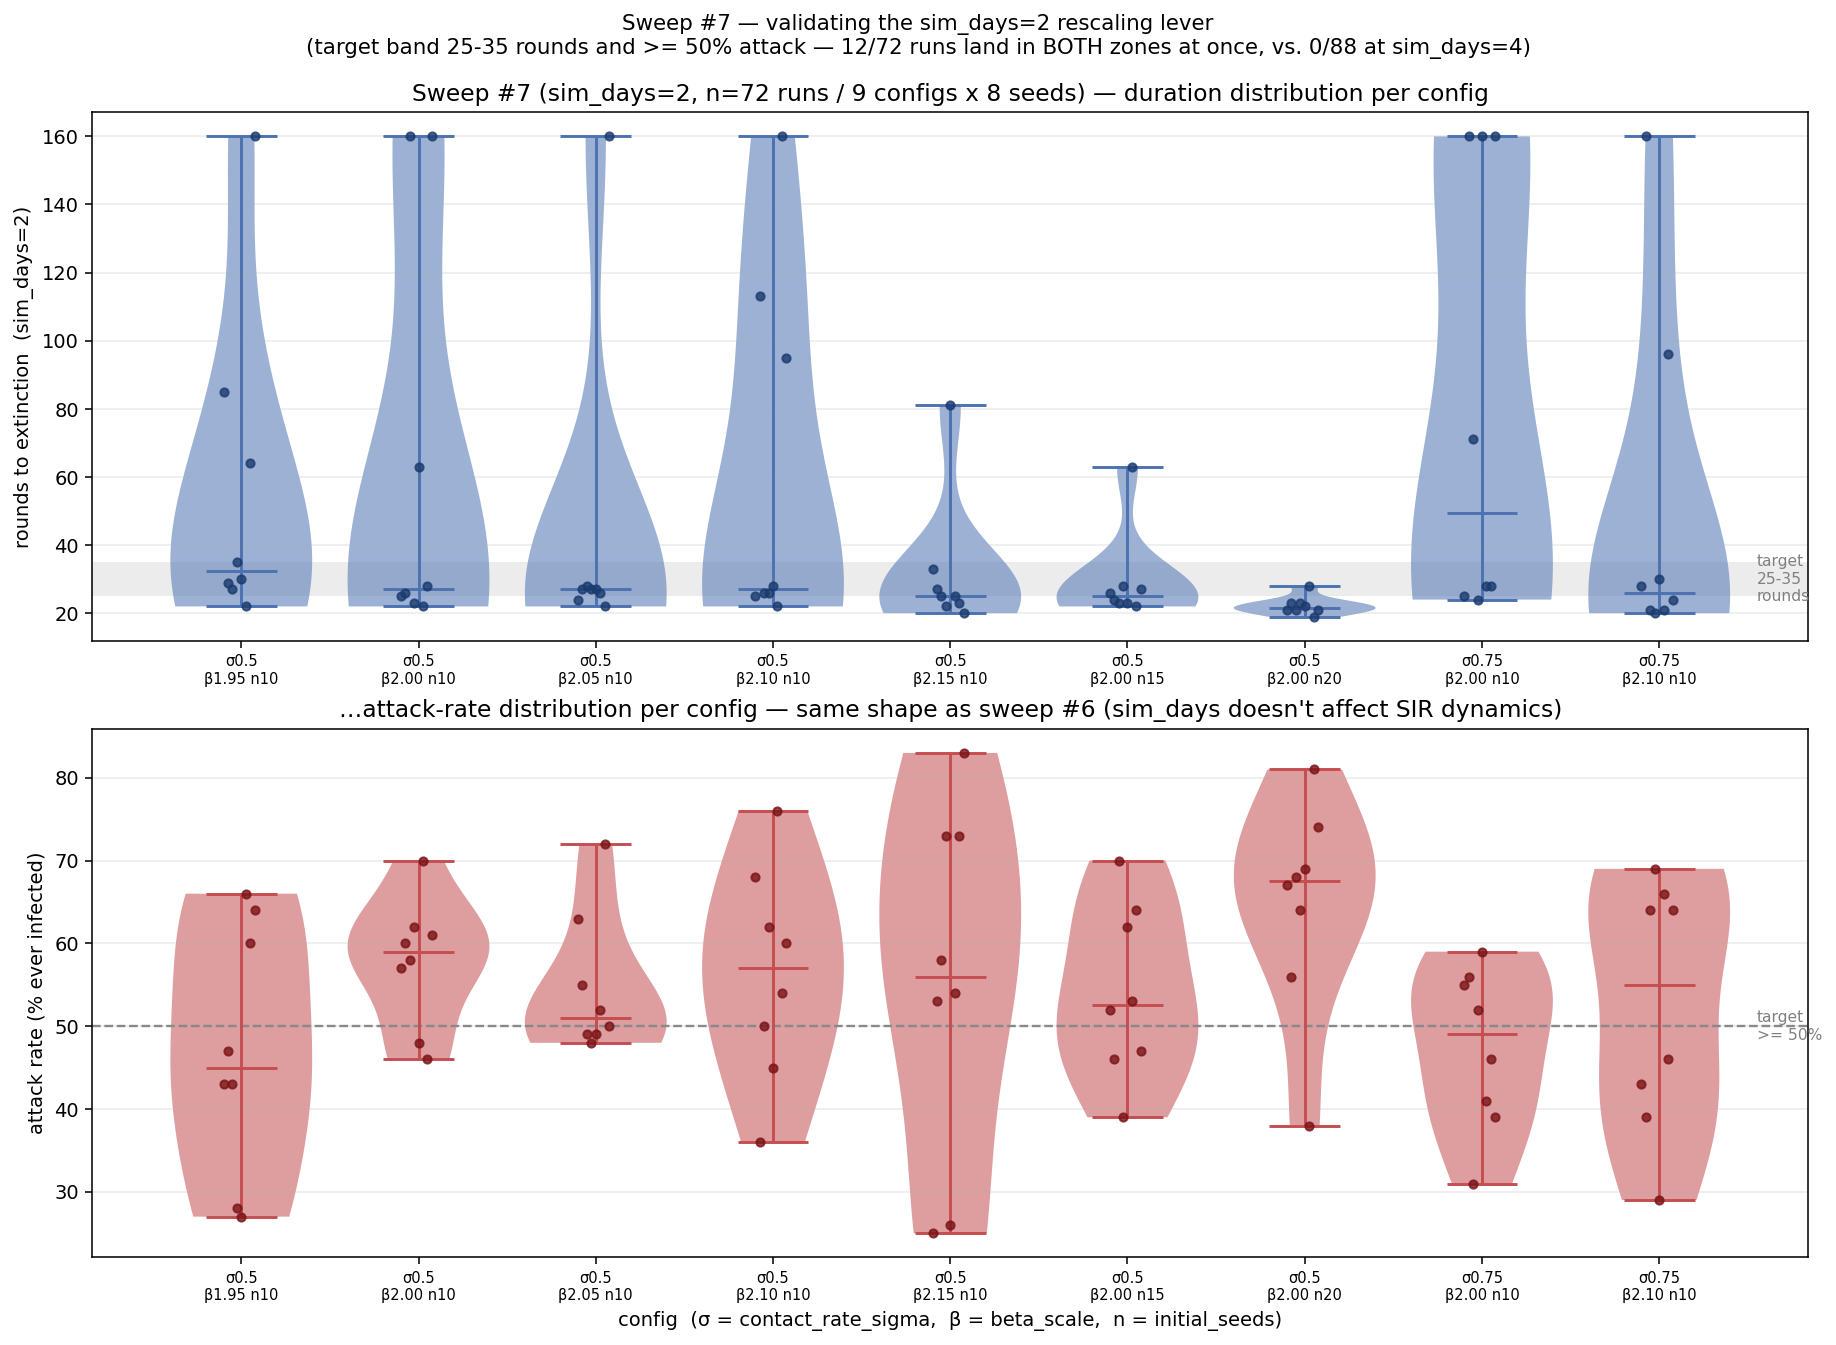
\includegraphics[width=0.9\textwidth]{sec2_fig7_sir_calibration_violins.png}
  \caption{SIR calibration sweep \#7 (\texttt{sim\_days=2}): violin plots of
  rounds-to-extinction (top) and final attack rate (bottom) across 9
  \texttt{(contact\_rate\_sigma, beta\_scale, initial\_seeds)} configurations,
  8 seeds each (72 runs). Shaded bands mark the target rounds-to-extinction
  window (25:35) and the target attack-rate floor ($\geq 50\%$).}
  \label{fig:sir-calibration-violins}
\end{figure}

At \texttt{sim\_days=2}, 9 configurations $\times$ 8 seeds (72 runs) were
evaluated against the joint target. 12/72 runs (17\%) landed inside both
bands; the best individual configuration ($\sigma=0.5$, $\beta=2.00$,
\texttt{initial\_seeds=10}) hit the joint target in 3/8 seeds, with median
27 rounds to extinction and median 59\% attack rate. The attack-rate
distribution by configuration has the same shape as an earlier sweep at
\texttt{sim\_days=4} (0/88 joint hits there), consistent with
\texttt{sim\_days} rescaling round-count without altering attack rate. The
adopted production configuration for the live-SIR FL run reported in the
main text is $\sigma=0.5$, $\beta=2.00$, \texttt{initial\_seeds=10},
\texttt{sim\_days=2}.


\section{Schedule-Shape Ablation Detail}
\label{sec:supp-schedule-ablation}

\subsection{Setup and Metrics}

\subsubsection{Data generation pipeline}

Each condition fixes 3 silos $\times$ 3 diseases. Two text generators:
\begin{itemize}
  \item \textbf{template}: fill-in-the-blank symptom sentences with per-disease vocabulary
  \item \textbf{phrase\_library}: richer lexical diversity drawn from a curated phrase bank
\end{itemize}

Two label distributions:
\begin{itemize}
  \item \textbf{IID}: each silo sees all 3 diseases equally
  \item \textbf{Non-IID}: silos are disease-biased (each has a dominant disease at 60\%, others at 20\%)
\end{itemize}

\subsubsection{Volume schedule}

Every condition delivers exactly \textbf{160 events per silo per run} (20
rounds $\times$ 8 events/round average). The five schedule shapes vary
\emph{when} those events arrive --- but total volume is matched. This
isolates temporal distribution from data quantity.

\subsubsection{Key metrics}

\begin{table}[H]
  \centering
  \caption{Metrics logged per FL round.}
  \begin{tabular}{ll}
    \toprule
    Metric & Description \\
    \midrule
    \texttt{n\_reveal} & Events revealed to each silo in that round (list of 3) \\
    \texttt{mean\_loss} & FedAvg global training loss over the round's batches \\
    \texttt{agg\_diag\_acc} & Global (averaged) diagnostic accuracy on held-out probe set \\
    \texttt{silo\_diag[i]} & Per-silo diagnostic accuracy (measures local specialisation) \\
    \bottomrule
  \end{tabular}
\end{table}

\textbf{Theoretical bounds:} Bayes floor $\approx 0.10$
(\texttt{confusion\_rate}), empirical ceiling $\approx 0.88$--$0.93$ with
template generator, $\approx 0.85$--$0.93$ with phrase\_library (harder
task).

\subsection{Schedule Shapes}

All five shapes deliver 160 events over 20 rounds; they differ in temporal
concentration:

\begin{table}[H]
  \centering
  \caption{Schedule shape definitions.}
  \begin{tabular}{lll}
    \toprule
    Shape & Character & Peak rounds \\
    \midrule
    flat & Uniform 8 events/round throughout & all \\
    gaussian & Bell curve centred at round 10 & $r\approx7$--13 \\
    burst & Heavily front-loaded, rapid decay & $r=1$--4 \\
    ramp & Linearly increasing & $r=16$--20 \\
    parabola (U) & Concave: heavy at start and end, sparse in middle & $r=1$--3, $r=17$--20 \\
    \bottomrule
  \end{tabular}
\end{table}


\subsubsection{Template generator}

The template generator produces fill-in-the-blank symptom narratives
from a fixed per-disease vocabulary, with no LLM involvement.
Figures~\ref{fig:supp-per-shape-template-iid}
and~\ref{fig:supp-per-shape-template-noniid} show training loss and
diagnostic accuracy curves across all five schedule shapes under IID and
Non-IID label distributions respectively.

\paragraph{IID distribution.}
Under IID conditions each silo receives all three diseases in equal
proportion, so silos converge from the same starting distribution.
\begin{figure}[H]
  \centering
  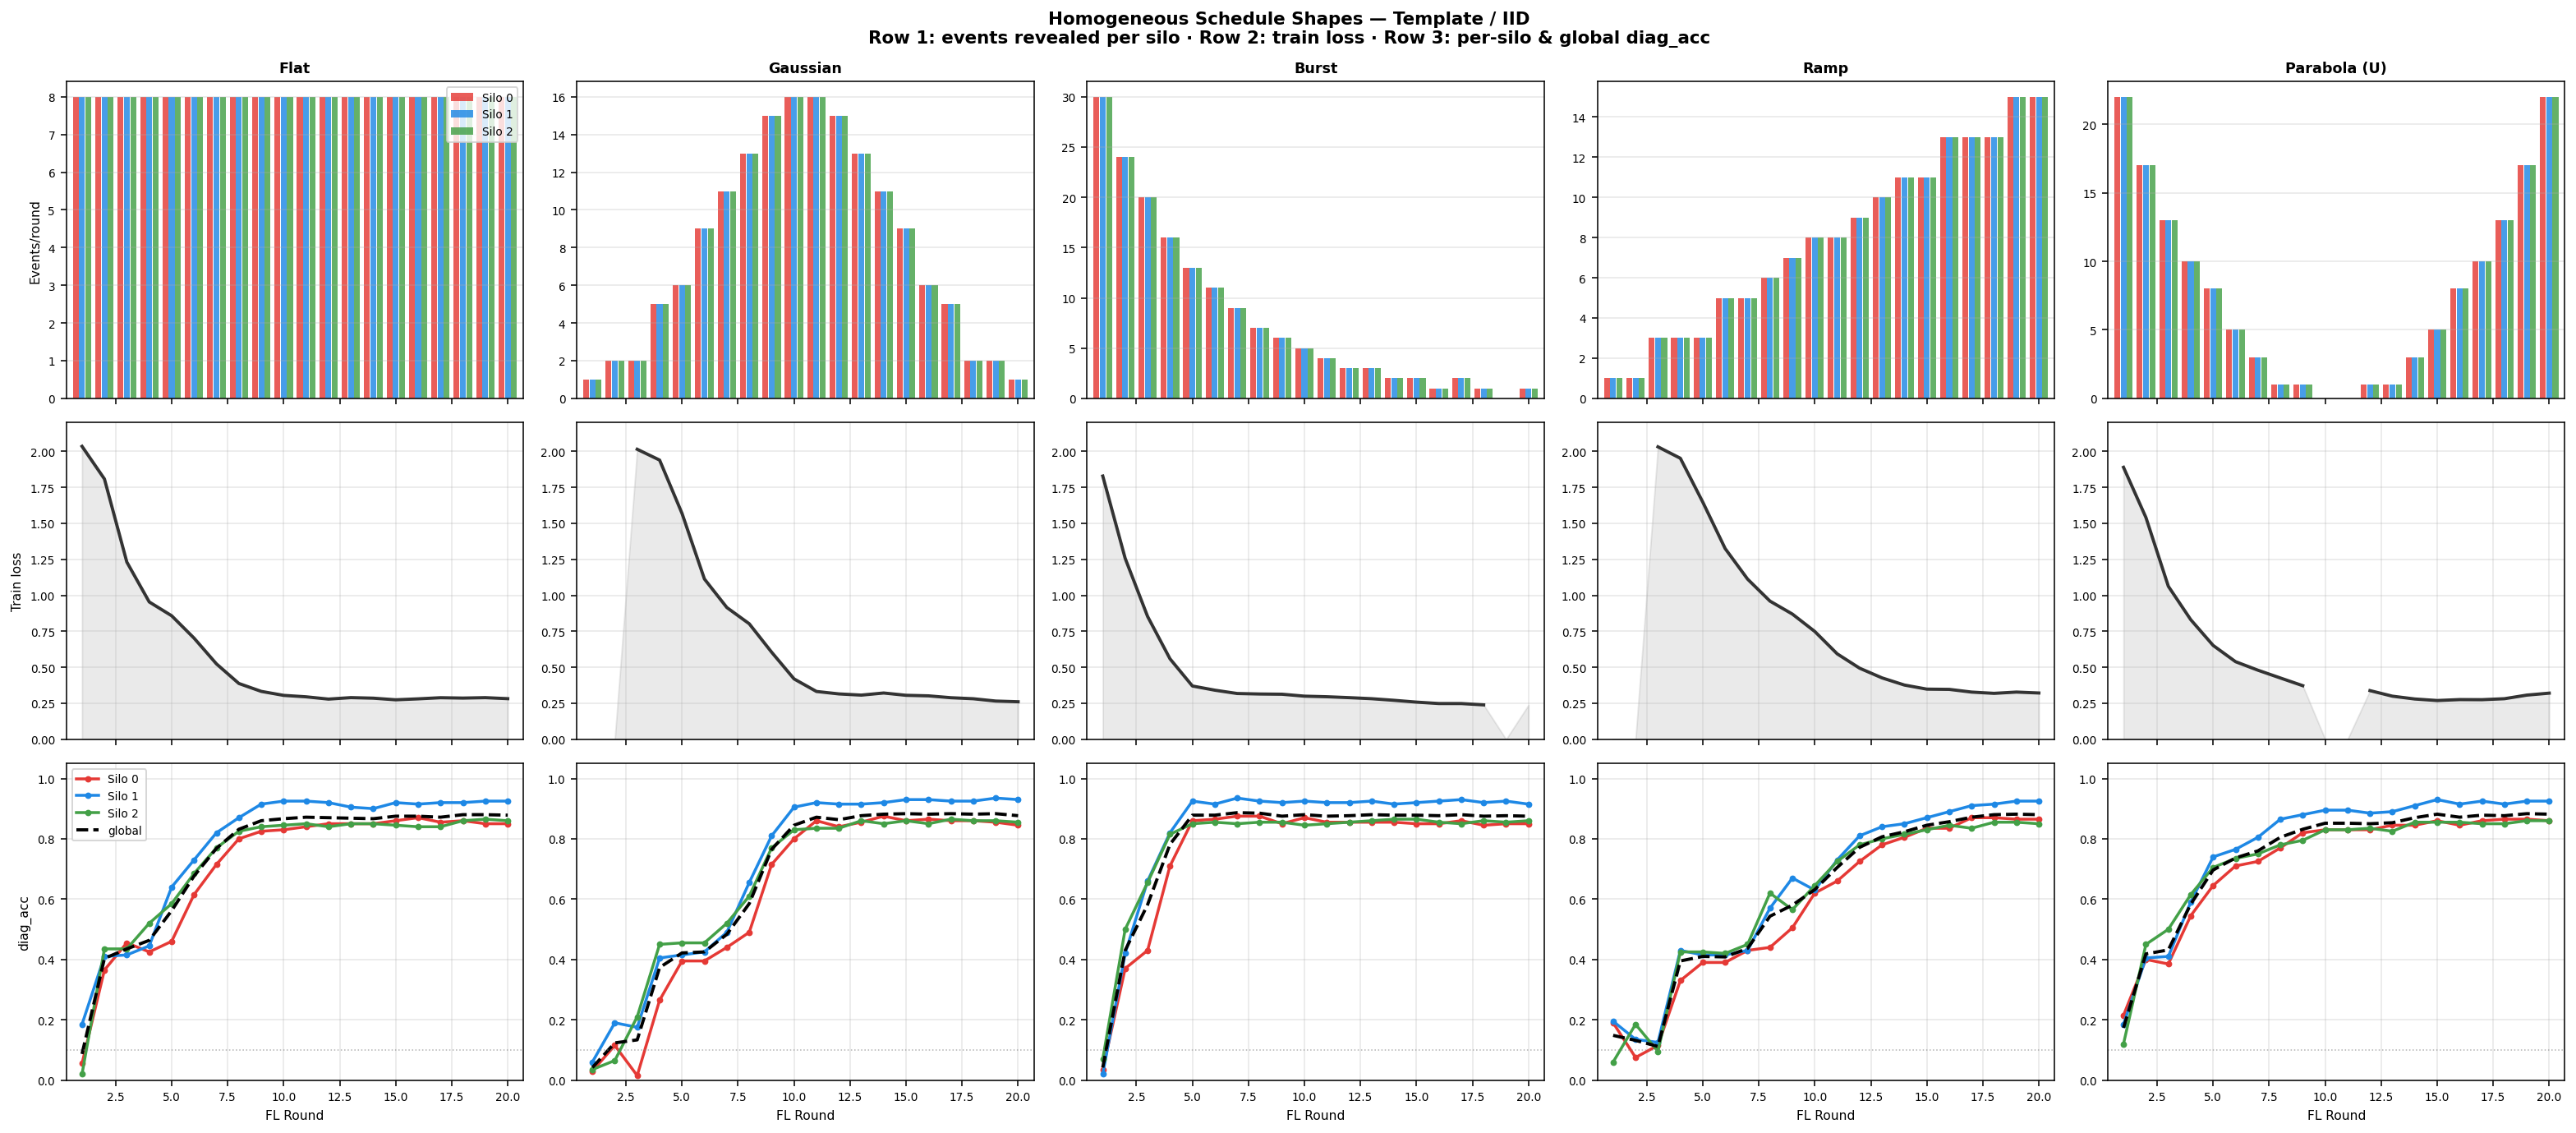
\includegraphics[width=0.9\textwidth]{sec2_fig8_per_shape_template_iid.png}
  \caption{Homogeneous shapes --- template / IID.}
  \label{fig:supp-per-shape-template-iid}
\end{figure}

\paragraph{Non-IID distribution.}
Under Non-IID conditions each silo has a dominant disease at 60\%,
with the remaining 40\% split across the other two; silos therefore
specialise before federation balances them out.
\begin{figure}[H]
  \centering
  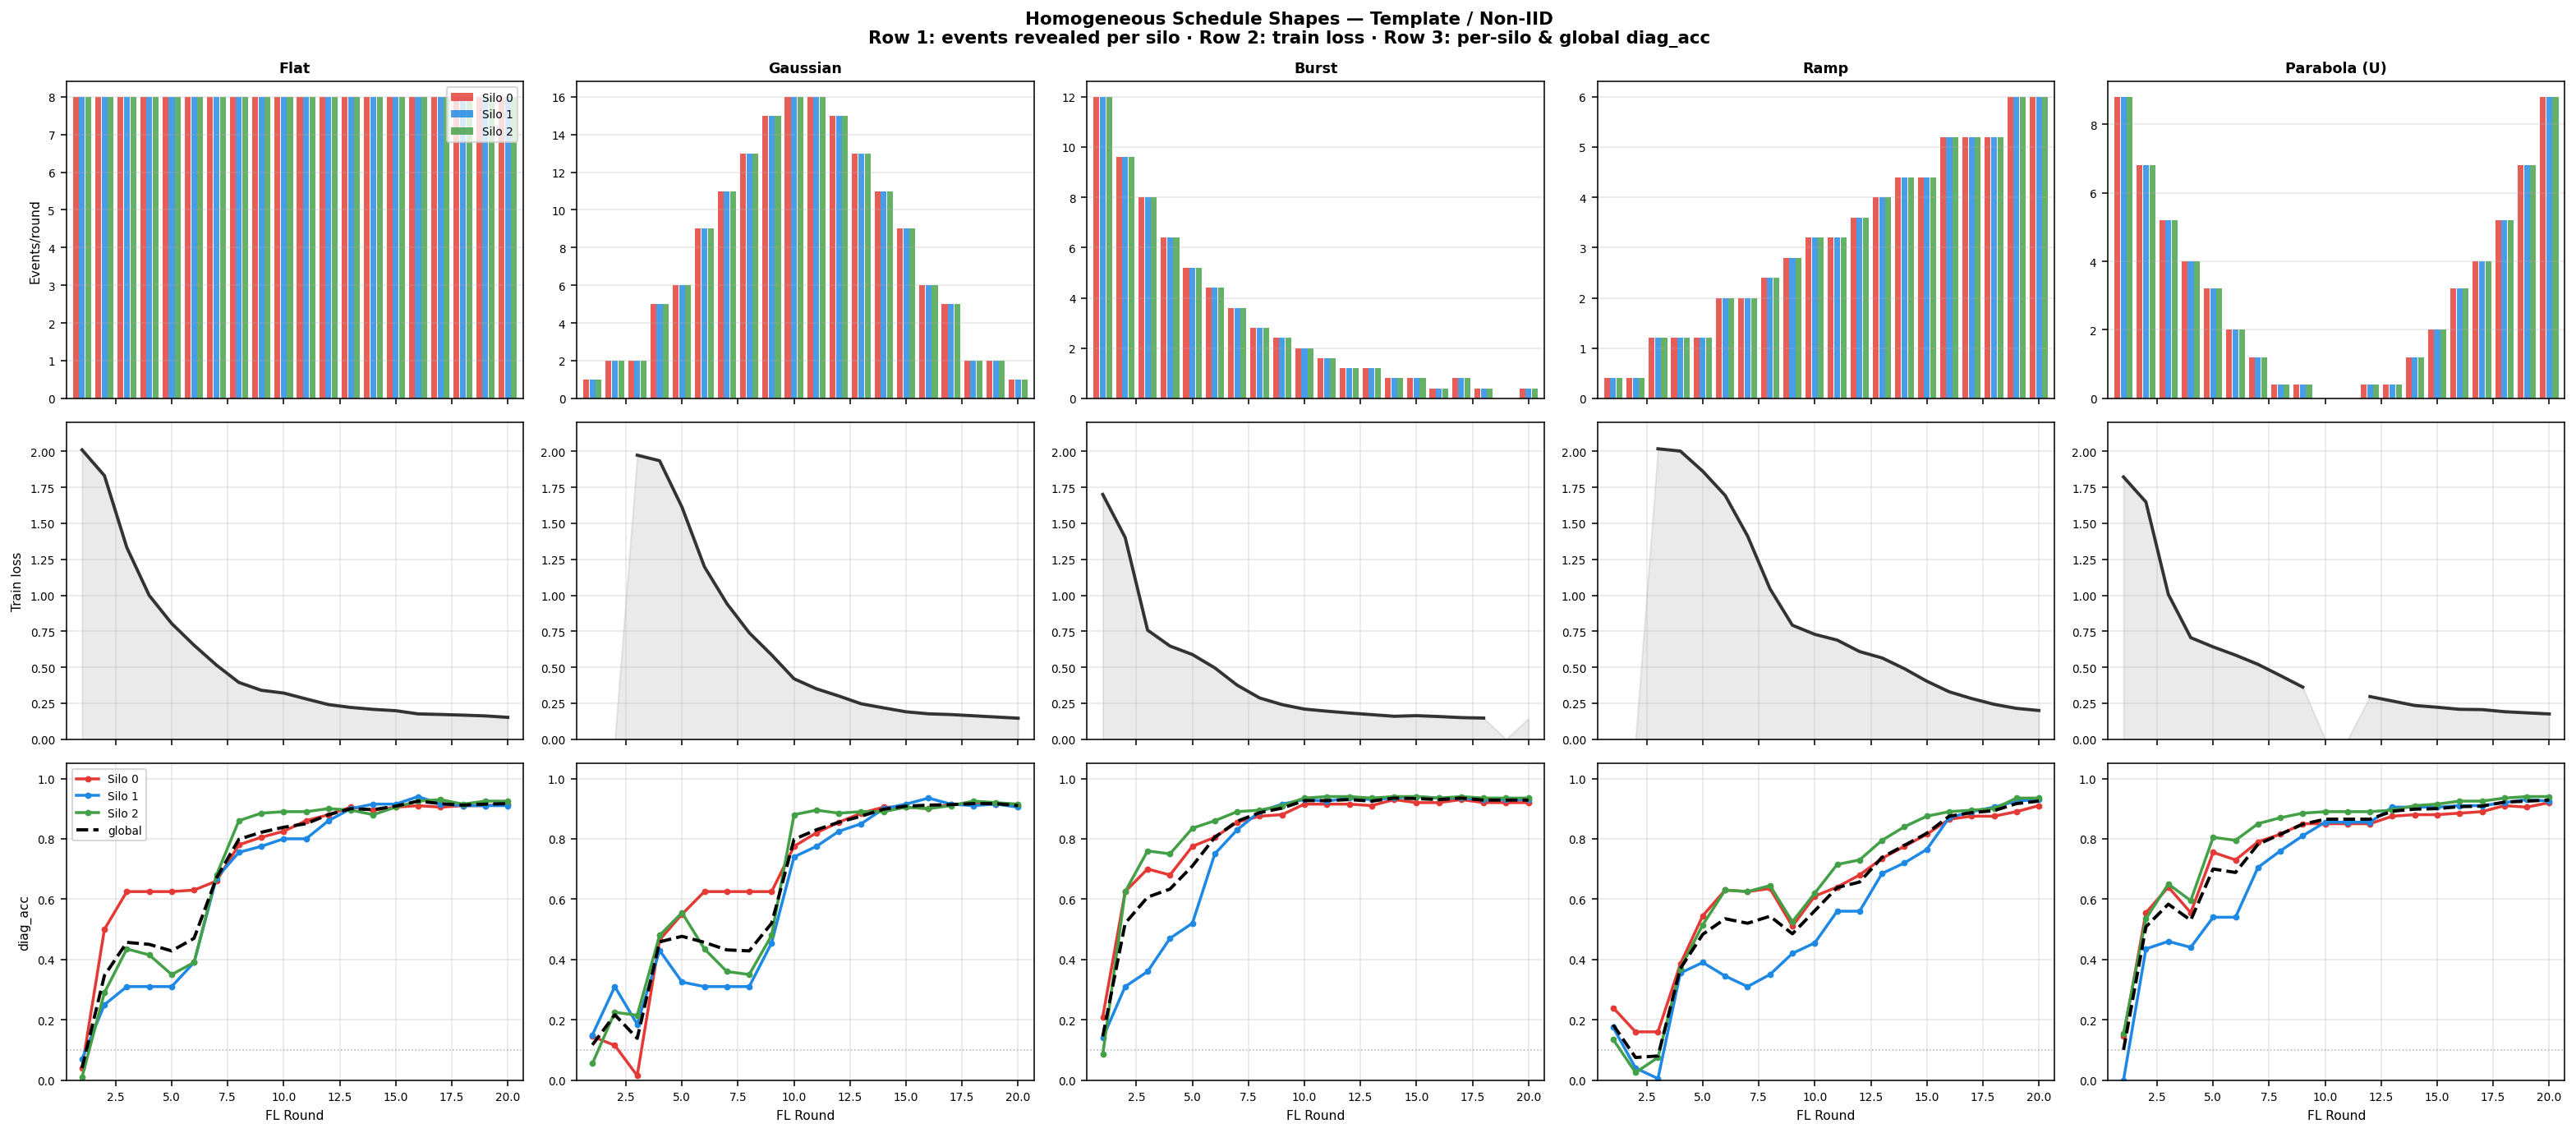
\includegraphics[width=0.9\textwidth]{sec2_fig9_per_shape_template_noniid.png}
  \caption{Homogeneous shapes --- template / Non-IID.}
  \label{fig:supp-per-shape-template-noniid}
\end{figure}

\subsubsection{Phrase-library generator}

The phrase-library generator draws from a curated bank of natural
symptom expressions, producing higher lexical diversity at the cost of
a noisier signal.
Figures~\ref{fig:supp-per-shape-phraselib-iid}
and~\ref{fig:supp-per-shape-phraselib-noniid} repeat the same schedule
comparison under this harder text regime.

\paragraph{IID distribution.}
\begin{figure}[H]
  \centering
  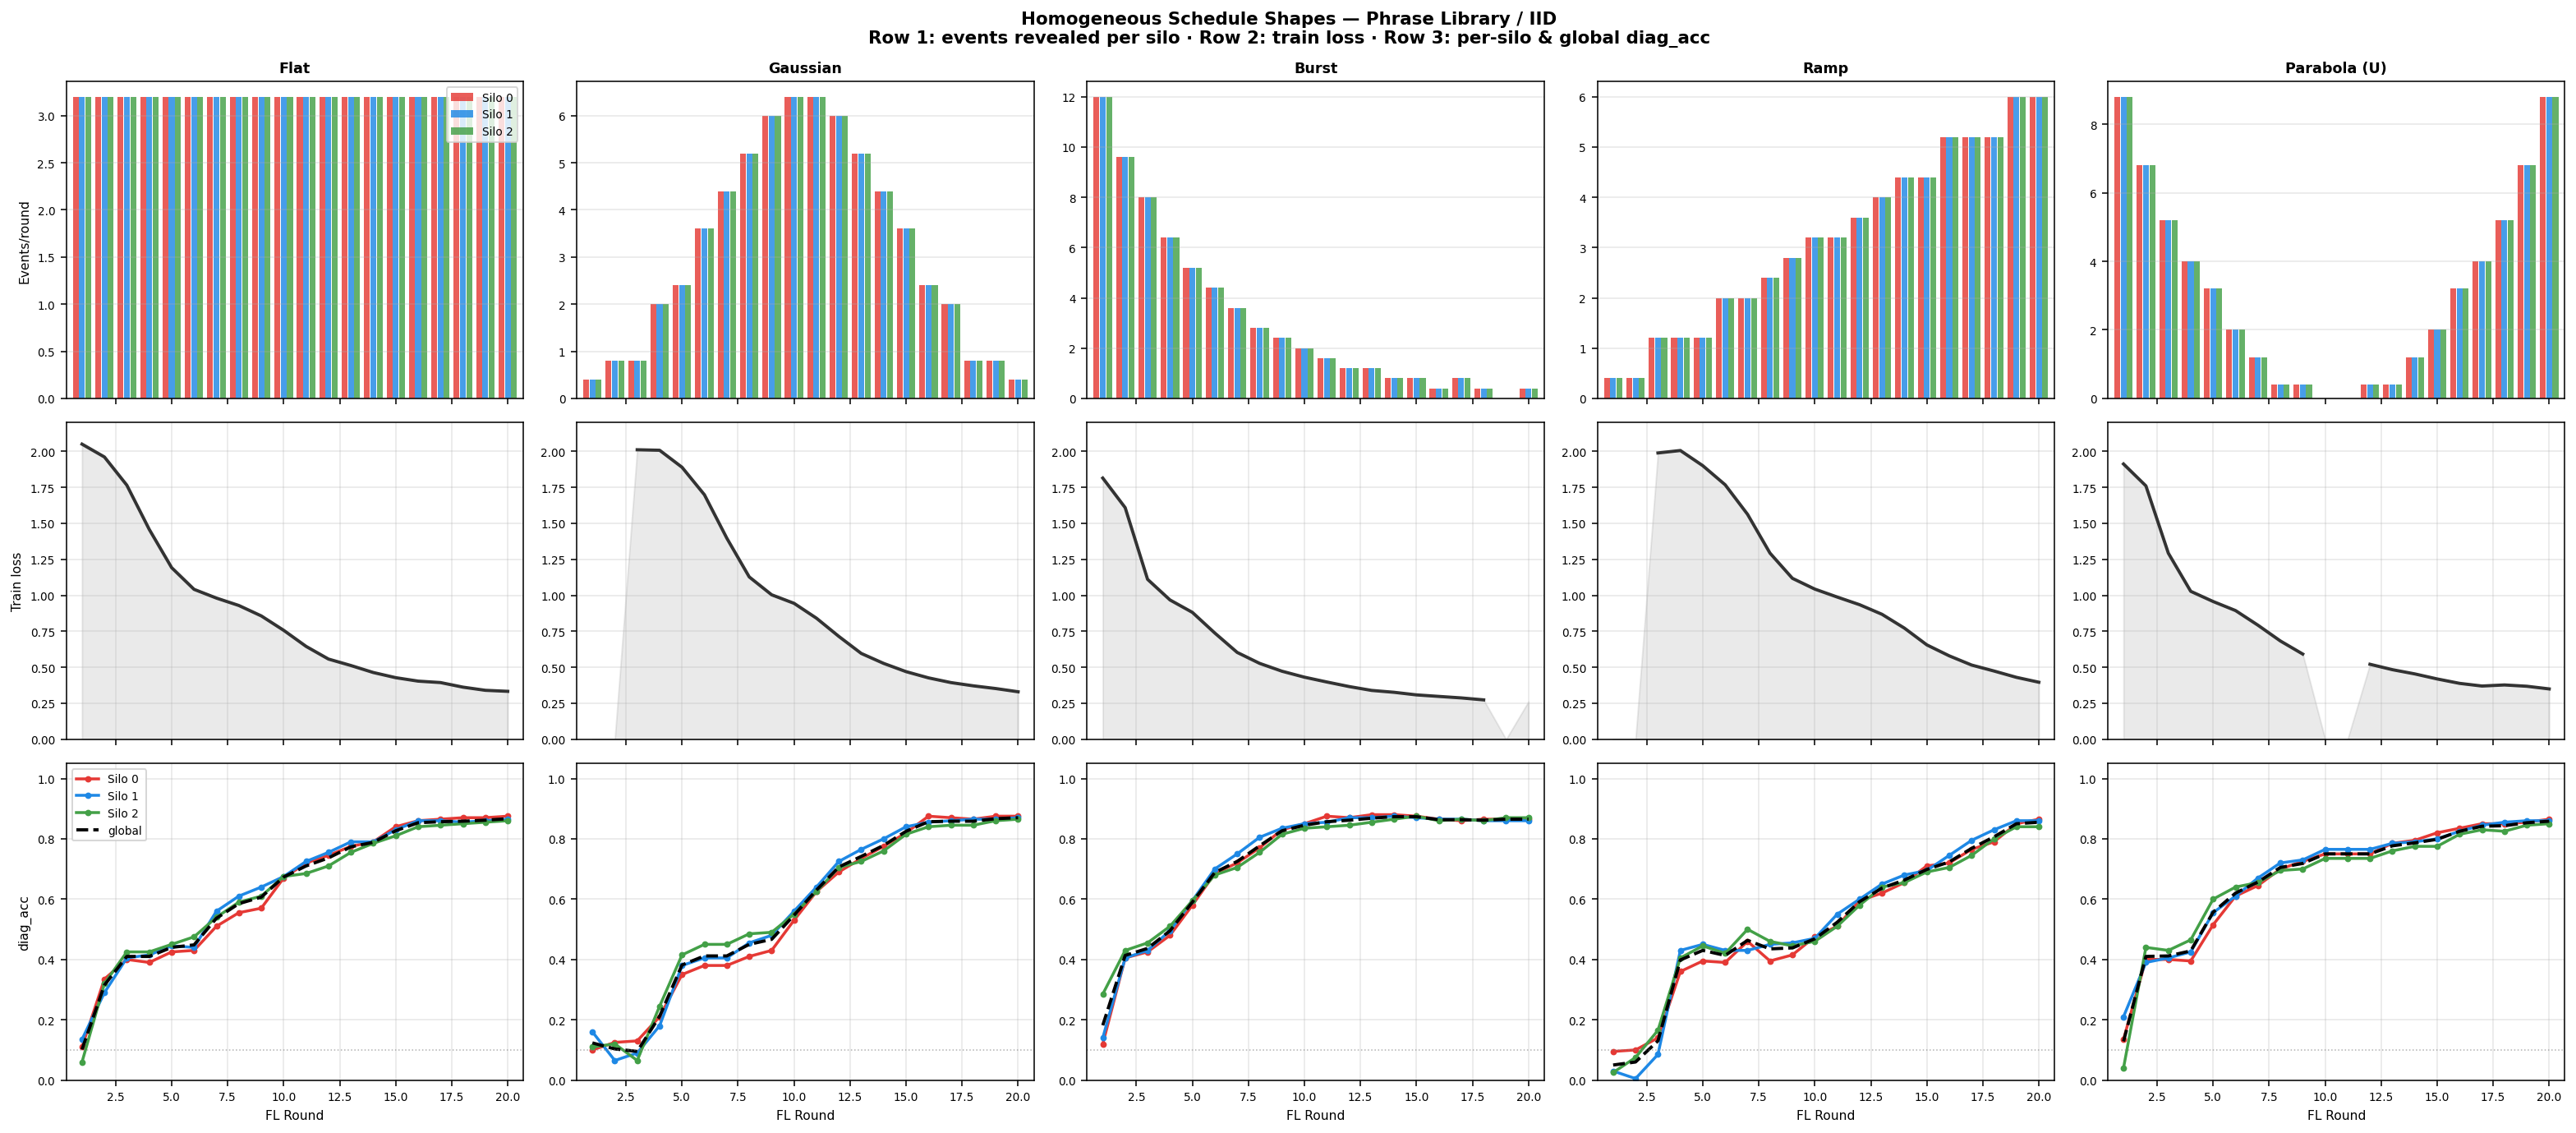
\includegraphics[width=0.9\textwidth]{sec2_fig10_per_shape_phrase_library_iid.png}
  \caption{Homogeneous shapes --- phrase\_library / IID.}
  \label{fig:supp-per-shape-phraselib-iid}
\end{figure}

\paragraph{Non-IID distribution.}
\begin{figure}[H]
  \centering
  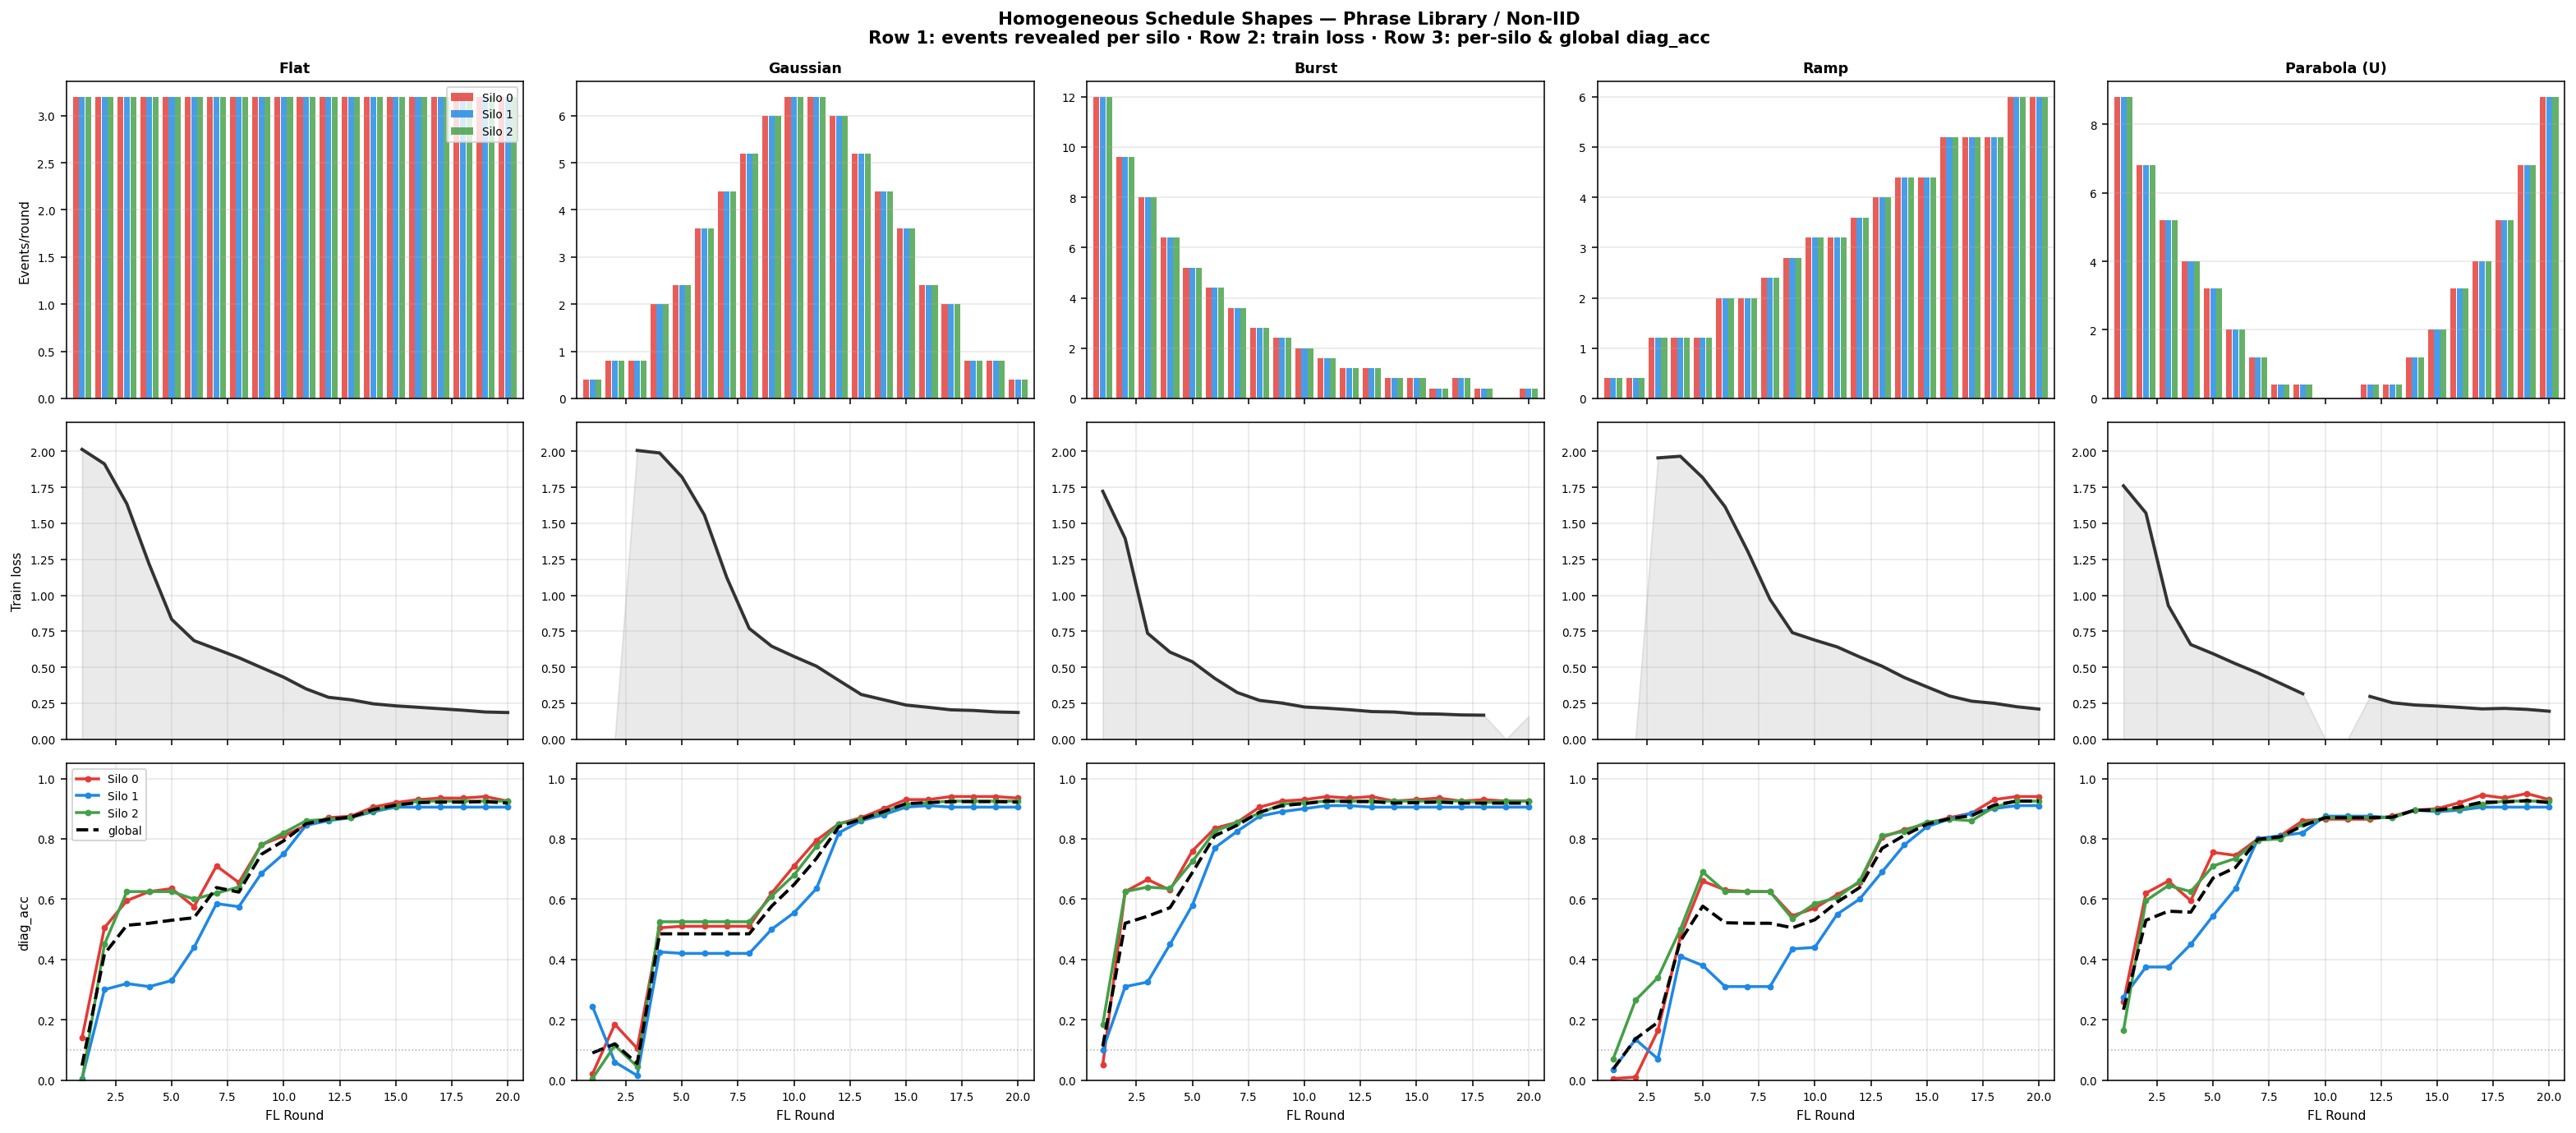
\includegraphics[width=0.9\textwidth]{sec2_fig11_per_shape_phrase_library_noniid.png}
  \caption{Homogeneous shapes --- phrase\_library / Non-IID.}
  \label{fig:supp-per-shape-phraselib-noniid}
\end{figure}

\subsubsection{Peak accuracy table --- homogeneous schedules (n=5 seeds, mean$\pm$std)}

\begin{table}[H]
  \centering
  \caption{Peak diagnostic accuracy by schedule shape, homogeneous schedules.}
  \begin{tabular}{lrrrr}
    \toprule
    Schedule & TMP/IID & TMP/Non-IID & PL/IID & PL/Non-IID \\
    \midrule
    flat      & $0.892\pm0.012$ & $0.930\pm0.023$ & $0.868\pm0.016$ & $0.923\pm0.032$ \\
    gaussian  & $0.892\pm0.016$ & $0.927\pm0.021$ & $0.872\pm0.019$ & $0.923\pm0.031$ \\
    burst     & $0.897\pm0.011$ & $0.937\pm0.024$ & $0.882\pm0.022$ & $0.925\pm0.030$ \\
    ramp      & $0.888\pm0.019$ & $0.925\pm0.020$ & $0.857\pm0.017$ & $0.927\pm0.028$ \\
    parabola  & $0.888\pm0.011$ & $0.930\pm0.020$ & $0.860\pm0.016$ & $0.927\pm0.028$ \\
    \bottomrule
  \end{tabular}
  \label{tab:supp-peak-acc-by-shape}
\end{table}

\subsubsection{Observations}

\begin{itemize}
  \item \textbf{All five shapes converge to statistically indistinguishable
  accuracy.} The maximum spread across shapes is $\leq 0.009$ (within a
  single generator $\times$ distribution cell). No schedule shape
  systematically outperforms any other when total data volume is matched.
  \item \textbf{Burst} shows the fastest early loss drop (loss $< 1.0$ by
  round 5) because the model receives 30--40 events in rounds 1--3, before
  the other shapes have ramped up. However, the benefit does not persist
  --- by round 20 all shapes converge.
  \item \textbf{Ramp} is the opposite: high early loss, steeper drop in
  rounds 15--20 as events accumulate. Useful for simulating slow epidemic
  growth.
  \item \textbf{Parabola (U-shape)} creates an interesting loss pattern ---
  two learning phases separated by a quiescent middle, but again final
  accuracy is identical.
  \item \textbf{Non-IID is consistently higher} than IID (by 0.03--0.06).
  This is because per-silo specialisation in the non-IID setting transfers
  well: each silo excels at its dominant disease, and the federated
  aggregate benefits from complementary expertise.
  \item \textbf{Phrase-library lags template} by 0.01--0.02 in IID, but
  nearly matches in non-IID. The richer, noisier text surface is harder to
  fit but encodes more generalisable features.
\end{itemize}

\section{C2: Isolated Silo Experiments on Different Domains}
\label{sec:supp-c2-domains}

The pattern is checked for domain-generality in MNIST
(Table~\ref{tab:mnist-c2-sweep}) and IMDB sentiment
(Table~\ref{tab:sentiment-c2-sweep}), both $n=3$ throughout; in both,
the federated/isolated gap is small and non-significant at every tested
volume ($p\geq 0.10$ in all but one MNIST comparison), consistent with
the disease-text result at matched seed count. We keep
Tables~\ref{tab:mnist-c2-sweep}--\ref{tab:sentiment-c2-sweep} and
Figures~\ref{fig:mnist-c2-sweep}--\ref{fig:sentiment-c2-sweep} in the
main text; they replicate rather than extend the disease-text finding,
so they are the first candidates to move to supplementary if a length
constraint makes that necessary.

\begin{figure}[ht]
  \centering
  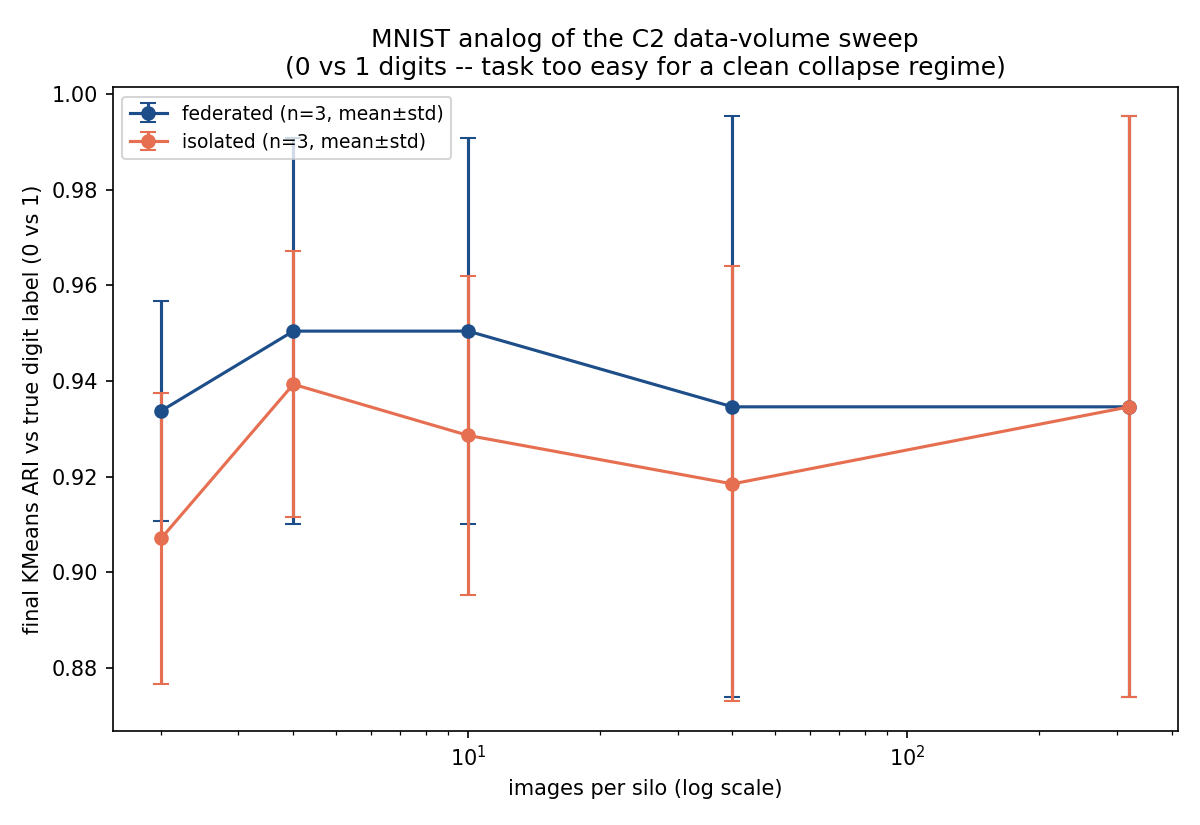
\includegraphics[width=0.9\textwidth]{sec5_act1_fig3_mnist_c2_data_volume_sweep.png}
  \caption{Federated and isolated ARI as a function of images per silo
  (2:320), MNIST domain.}
  \label{fig:mnist-c2-sweep}
\end{figure}

\begin{table}[ht]
  \centering
  \caption{C2 data-volume sweep, MNIST domain, $n=3$ seeds per point.}
  \begin{tabular}{rrrrr}
    \toprule
    Images/silo & Federated ARI & Isolated ARI & Gap & Exact perm.\ $p$ \\
    \midrule
    320 & $0.935 \pm 0.061$ & $0.935 \pm 0.061$ & $+0.000$ & 1.000 \\
    40  & $0.935 \pm 0.061$ & $0.918 \pm 0.045$ & $+0.016$ & 1.000 \\
    10  & $0.950 \pm 0.040$ & $0.929 \pm 0.033$ & $+0.022$ & 0.600 \\
    4   & $0.950 \pm 0.040$ & $0.939 \pm 0.028$ & $+0.011$ & 1.000 \\
    2   & $0.934 \pm 0.023$ & $0.907 \pm 0.030$ & $+0.027$ & 0.400 \\
    \bottomrule
  \end{tabular}
  \label{tab:mnist-c2-sweep}
\end{table}

\begin{figure}[ht]
  \centering
  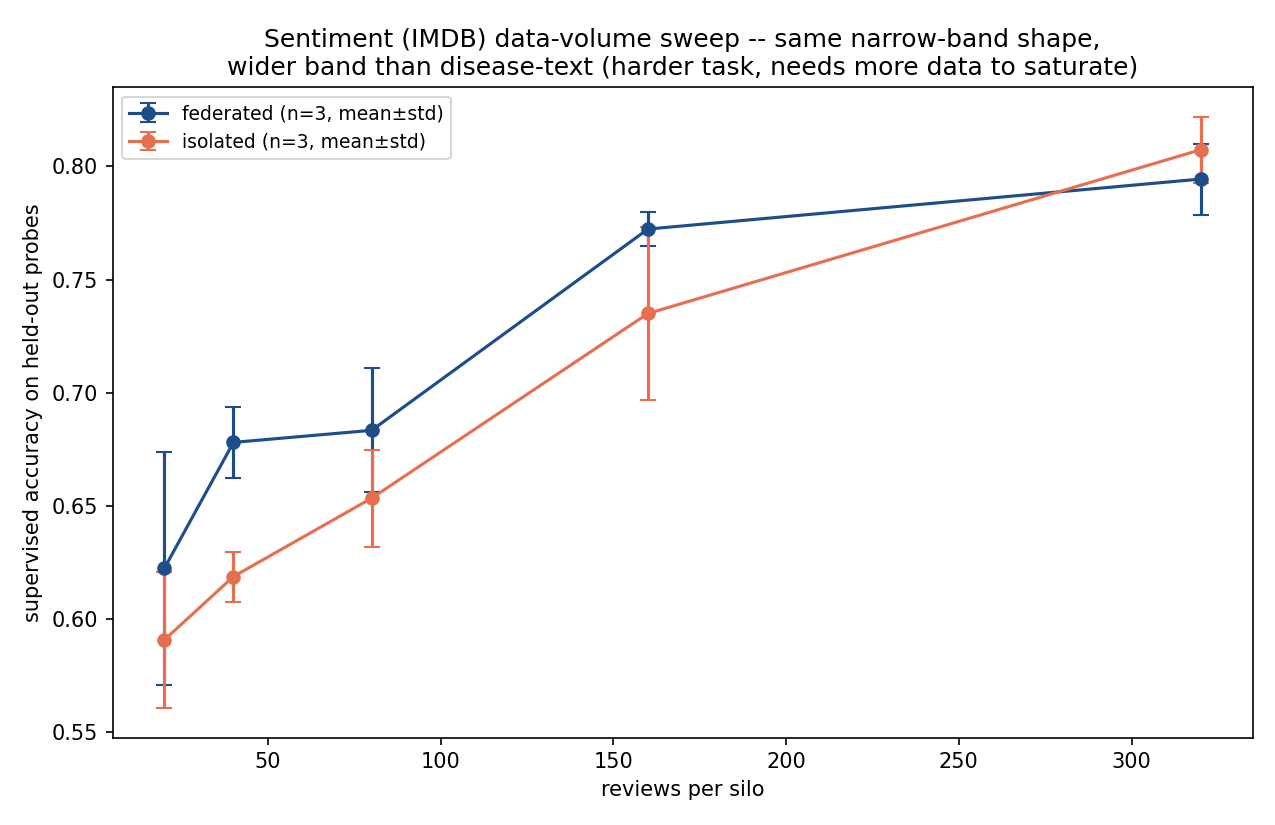
\includegraphics[width=0.9\textwidth]{sec5_act1_fig4_sentiment_c2_data_volume_sweep.png}
  \caption{Federated and isolated supervised classification accuracy as a
  function of reviews per silo (20:320), IMDB sentiment domain.}
  \label{fig:sentiment-c2-sweep}
\end{figure}

\begin{table}[ht]
  \centering
  \caption{C2 data-volume sweep, sentiment domain, $n=3$ seeds per point.
  Metric is supervised classification accuracy (unsupervised ARI on CLS
  embeddings was $\approx 0$ throughout this domain).}
  \begin{tabular}{rrrrr}
    \toprule
    Reviews/silo & Federated acc. & Isolated acc. & Gap & Exact perm.\ $p$ \\
    \midrule
    20  & $0.622 \pm 0.052$ & $0.591 \pm 0.030$ & $+0.031$ & 0.600 \\
    40  & $0.678 \pm 0.016$ & $0.619 \pm 0.011$ & $+0.059$ & 0.100 \\
    80  & $0.683 \pm 0.027$ & $0.654 \pm 0.021$ & $+0.030$ & 0.300 \\
    160 & $0.772 \pm 0.008$ & $0.735 \pm 0.039$ & $+0.037$ & 0.400 \\
    320 & $0.794 \pm 0.016$ & $0.807 \pm 0.015$ & $-0.013$ & --- \\
    \bottomrule
  \end{tabular}
  \label{tab:sentiment-c2-sweep}
\end{table}

\section{Aggregation Algorithm Exploration}
\label{sec:supp-aggregation}

The main text reports aggregate C4 false-positive rates at fixed
hyperparameters ($n=3$ seeds). This section provides a single-seed
hyperparameter scan to characterise sensitivity and confirm that the
ranking between algorithms is not an artifact of the default
parameterisation.

A single-seed hyperparameter scan (Figure~\ref{fig:aggregation-sweep})
provides exploratory context. FedProx's C4 FP rises monotonically with
$\mu$ ($0.0 \to 0.0 \to 0.194 \to 0.444$ for $\mu \in \{0.001, 0.01, 0.1,
1.0\}$), suggesting that tighter proximal regularization can recover
FedAvg-level accuracy. FedAdam is non-monotonic and collapses to $1.0$ once
server\_lr $\geq 0.1$, consistent with the bimodal instability seen in the
$n=3$ baseline. FedSGD's C4 FP is flat at $0.417$ across all tested learning
rates, indicating that its accuracy deficit is structural rather than a
hyperparameter artifact. Separately, reducing local\_epochs from $3$ to $1$
(single seed) does not alter the ranking: FedSGD remains consistently
elevated and FedAdam remains collapsed.

\begin{figure}[ht]
  \centering
  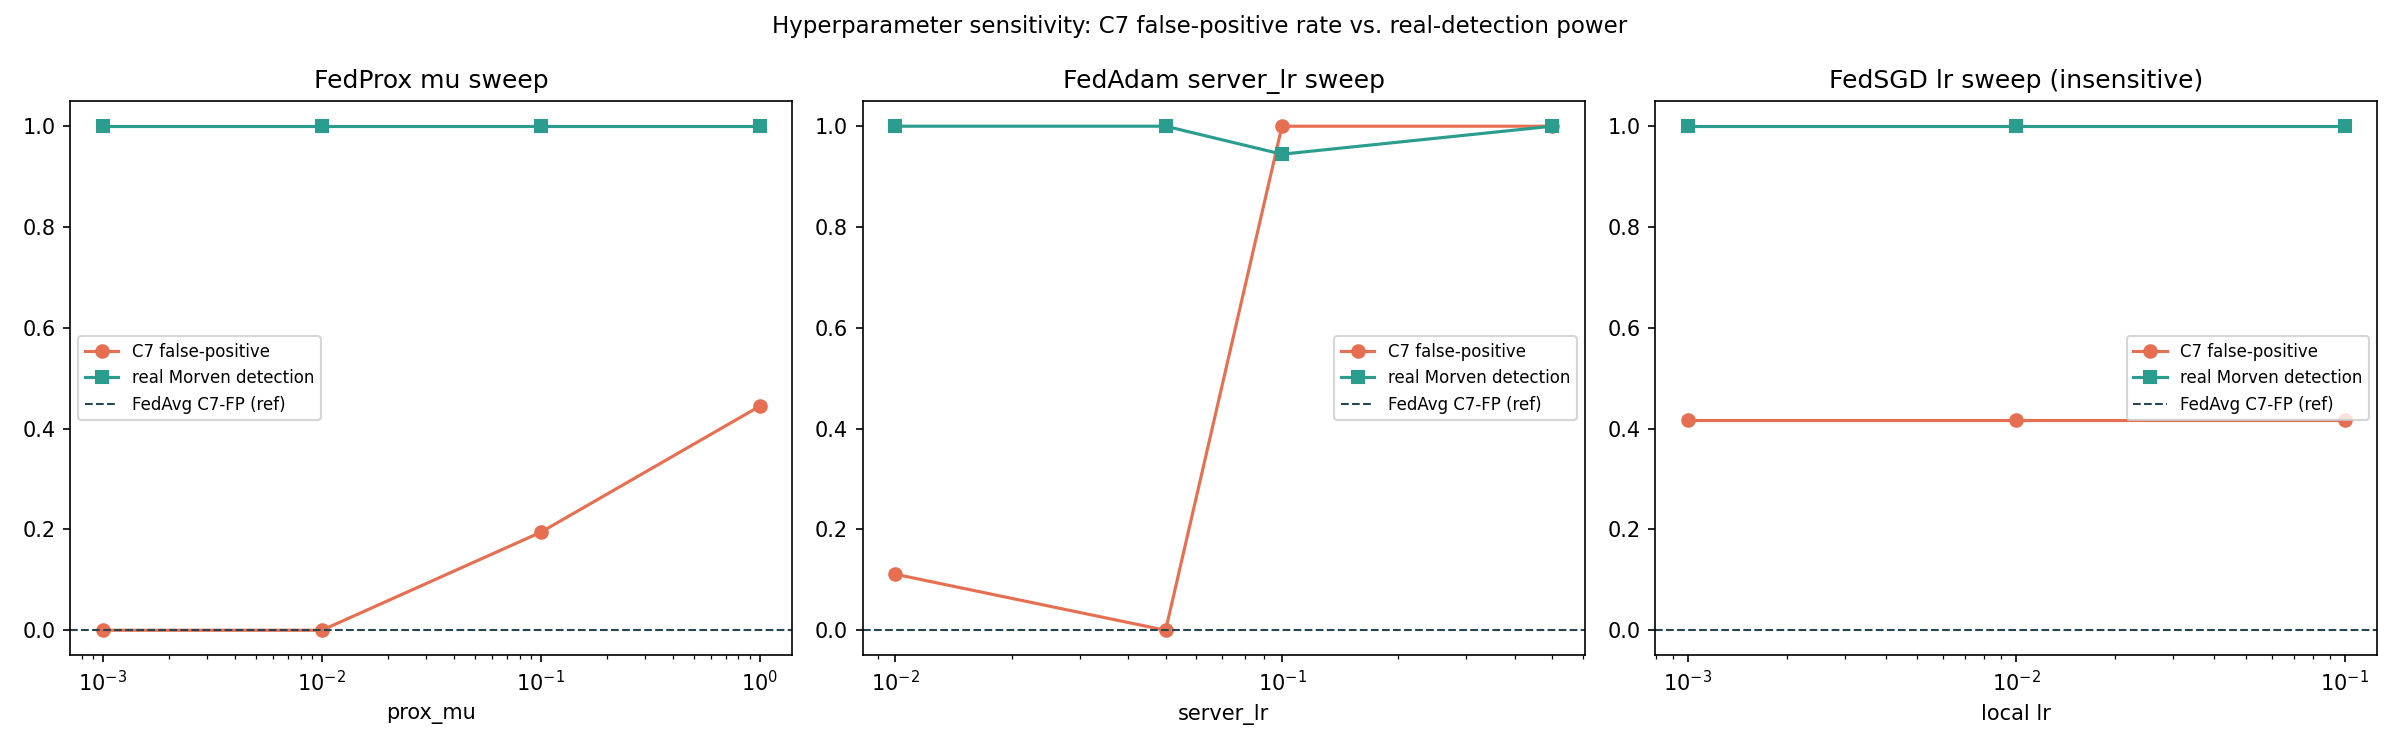
\includegraphics[width=0.9\textwidth]{sec5_act4_fig2_aggregation_sweep.png}
  \caption{Hyperparameter sensitivity, single seed per point: FedProx $\mu$,
  FedAdam server learning rate, FedSGD learning rate, against C4
  false-positive rate.}
  \label{fig:aggregation-sweep}
\end{figure}

\section{Cross-Domain Replication: MNIST}
\label{sec:supp-mnist-c4}

To confirm the detection/false-positive pattern is not specific to
disease-text, we replicate novel-class injection and the C4 control in
the MNIST handwritten digit dataset, holding out a digit as the novel
class (Table~\ref{tab:mnist-c4}). Known-digit leakage is low in both
scenarios ($\leq 0.056$), and novel recall is higher for genuinely novel
digits than for the relabeled-known control ($0.467 \pm 0.191$
vs.\ $0.256 \pm 0.110$): though the intervals overlap at $n=3$, so we
treat the direction as supportive rather than firmly established.

\begin{figure}[ht]
  \centering
  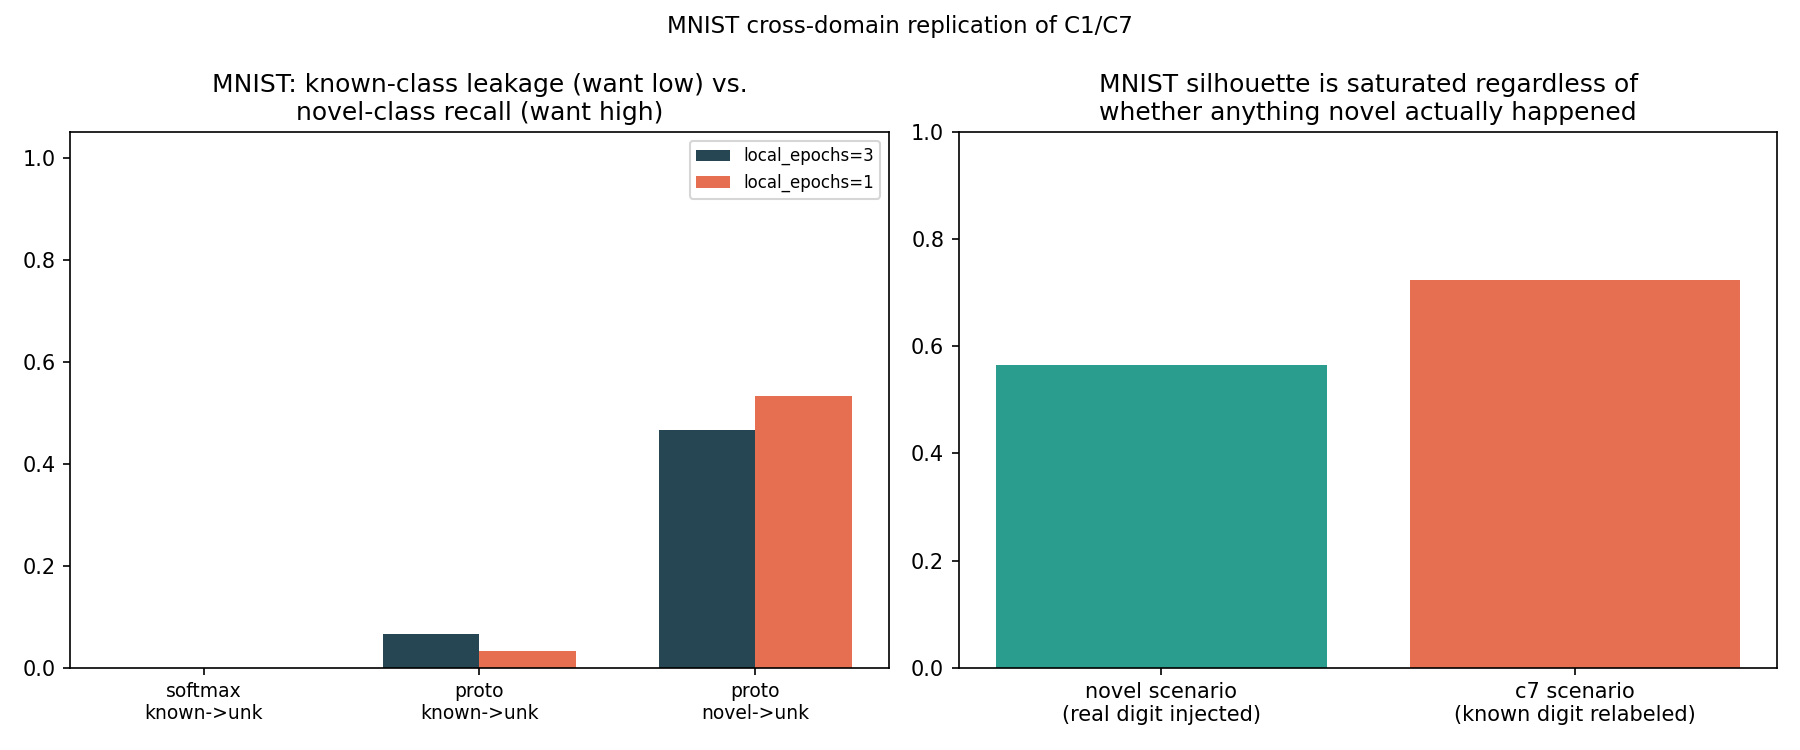
\includegraphics[width=0.9\textwidth]{sec5_act5_fig1_mnist_c7_comparison.png}
  \caption{MNIST domain: known-digit leakage and novel-digit recall, real
  novel-digit injection versus C4 known-digit-relabeled control, $n=3$ seeds.}
  \label{fig:mnist-c4-comparison}
\end{figure}

\begin{table}[ht]
  \centering
  \caption{MNIST C1/C4 replication, local\_epochs$=3$, $n=3$ seeds.}
  \begin{tabular}{lrr}
    \toprule
    Scenario & Known-digit leakage & Novel-digit recall \\
    \midrule
    \texttt{novel} (real digit injected) & $0.022 \pm 0.016$ & $0.467 \pm 0.191$ \\
    \texttt{c4} (known digit relabeled) & $0.056 \pm 0.016$ & $0.256 \pm 0.110$ \\
    \bottomrule
  \end{tabular}
  \label{tab:mnist-c4}
\end{table}

\section{Multilingual Silos}
\label{subsec:res-multilingual}

This subsection is exploratory and outside the falsification protocol of
the main text: a single heterogeneity axis (one language per silo) swept
at $n=1$ seed per condition, using
\texttt{distilbert-base-multilingual-cased} in place of the rest of the
paper's backbone. We report it as a single data point per condition, not
a validated finding, and flag it explicitly as a candidate for future
work requiring multi-seed replication before any directional claim
(e.g., about which languages transfer better) is drawn.

Figure~\ref{fig:bonus-volume-comparison} shows that disease-label ARI
improves with data volume and remains well above language-label ARI at
both tested volumes, confirming that the backbone organises embeddings
by disease identity rather than by silo language even in a multilingual
setting.

\begin{figure}[ht]
  \centering
  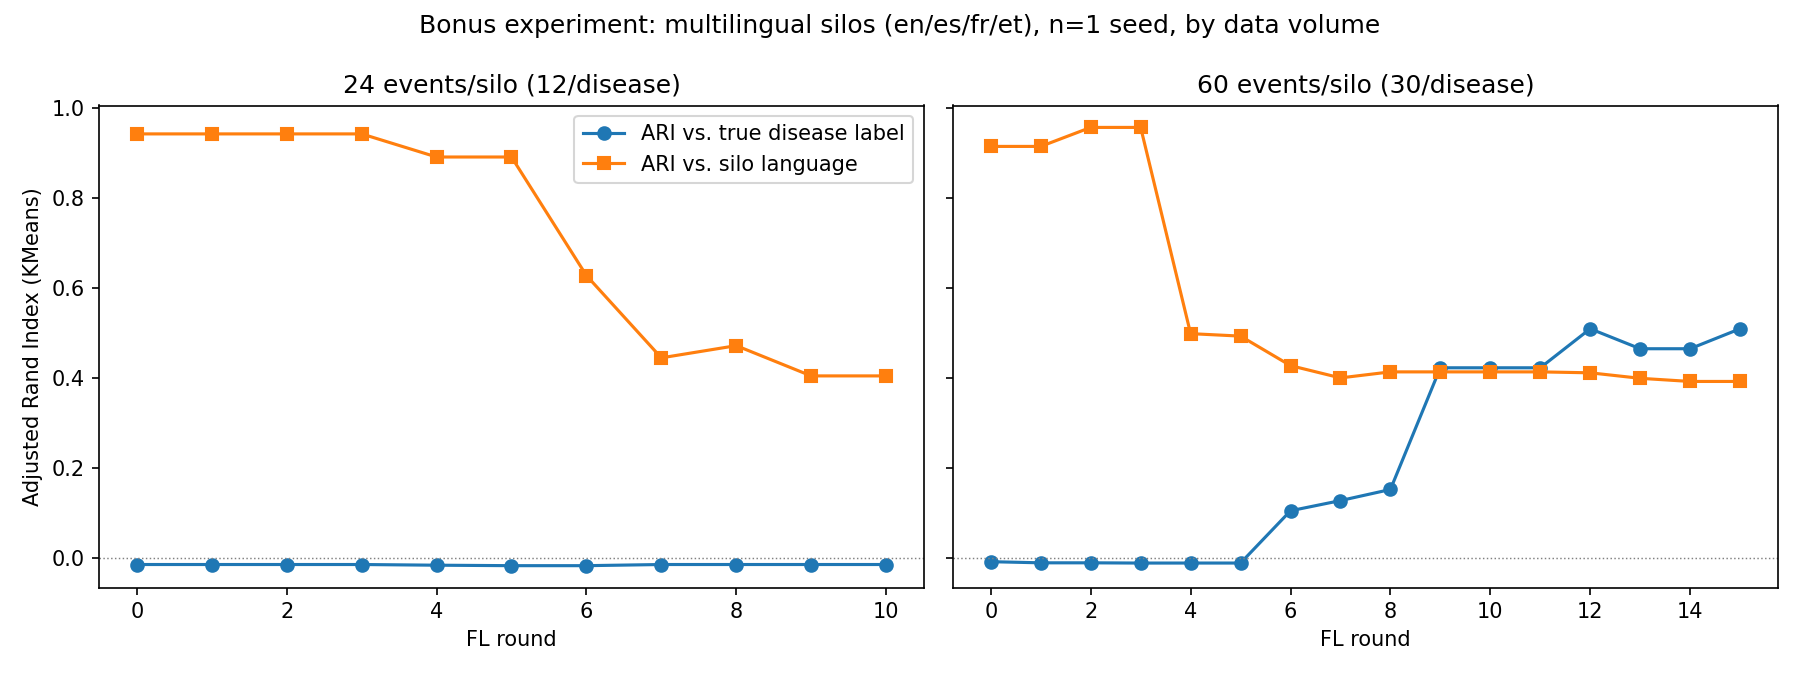
\includegraphics[width=0.95\textwidth]{bonus_fig1_multilingual_volume_comparison.png}
  \caption{Adjusted Rand Index vs.\ true disease label and vs.\ silo language,
  over FL rounds, four silos (English/Spanish/French/Estonian), at two data
  volumes: 24 events/silo (12/disease) and 60 events/silo (30/disease).}
  \label{fig:bonus-volume-comparison}
\end{figure}

Figure~\ref{fig:bonus-accuracy} breaks out supervised diagnostic accuracy
by language and shows that the global model achieves high overall accuracy
by round 15, though per-language performance diverges at $n=1$.

\begin{figure}[ht]
  \centering
  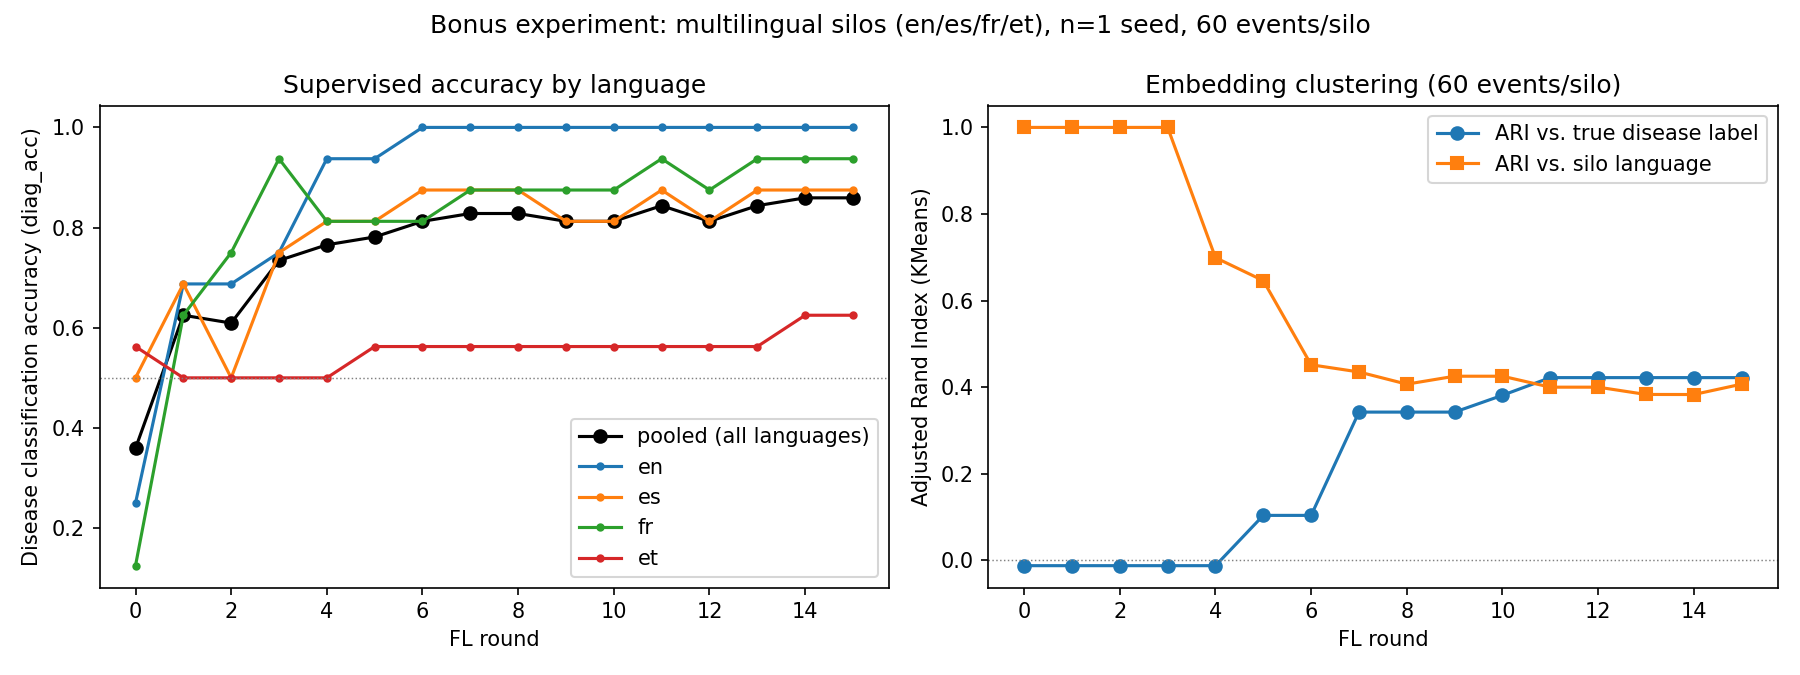
\includegraphics[width=0.95\textwidth]{bonus_fig2_multilingual_accuracy.png}
  \caption{Left: supervised disease-classification accuracy
  (\texttt{diag\_acc}) over FL rounds, pooled and broken out by language
  (en/es/fr/et), 60 events/silo. Right: the same run's ARI vs.\ disease and
  vs.\ language, for reference.}
  \label{fig:bonus-accuracy}
\end{figure}

At a single seed, English reaches perfect accuracy while Estonian lags
substantially (0.625); we do not attribute this to language identity
itself rather than to seed-specific variance, sample-size differences
within the multilingual backbone's pretraining corpus, or chance, given
$n=1$.

Figure~\ref{fig:bonus-global-clusters} shows the final-round UMAP of
global-model probe embeddings, confirming that clusters are aligned with
disease identity rather than silo language.

\begin{figure}[ht]
  \centering
  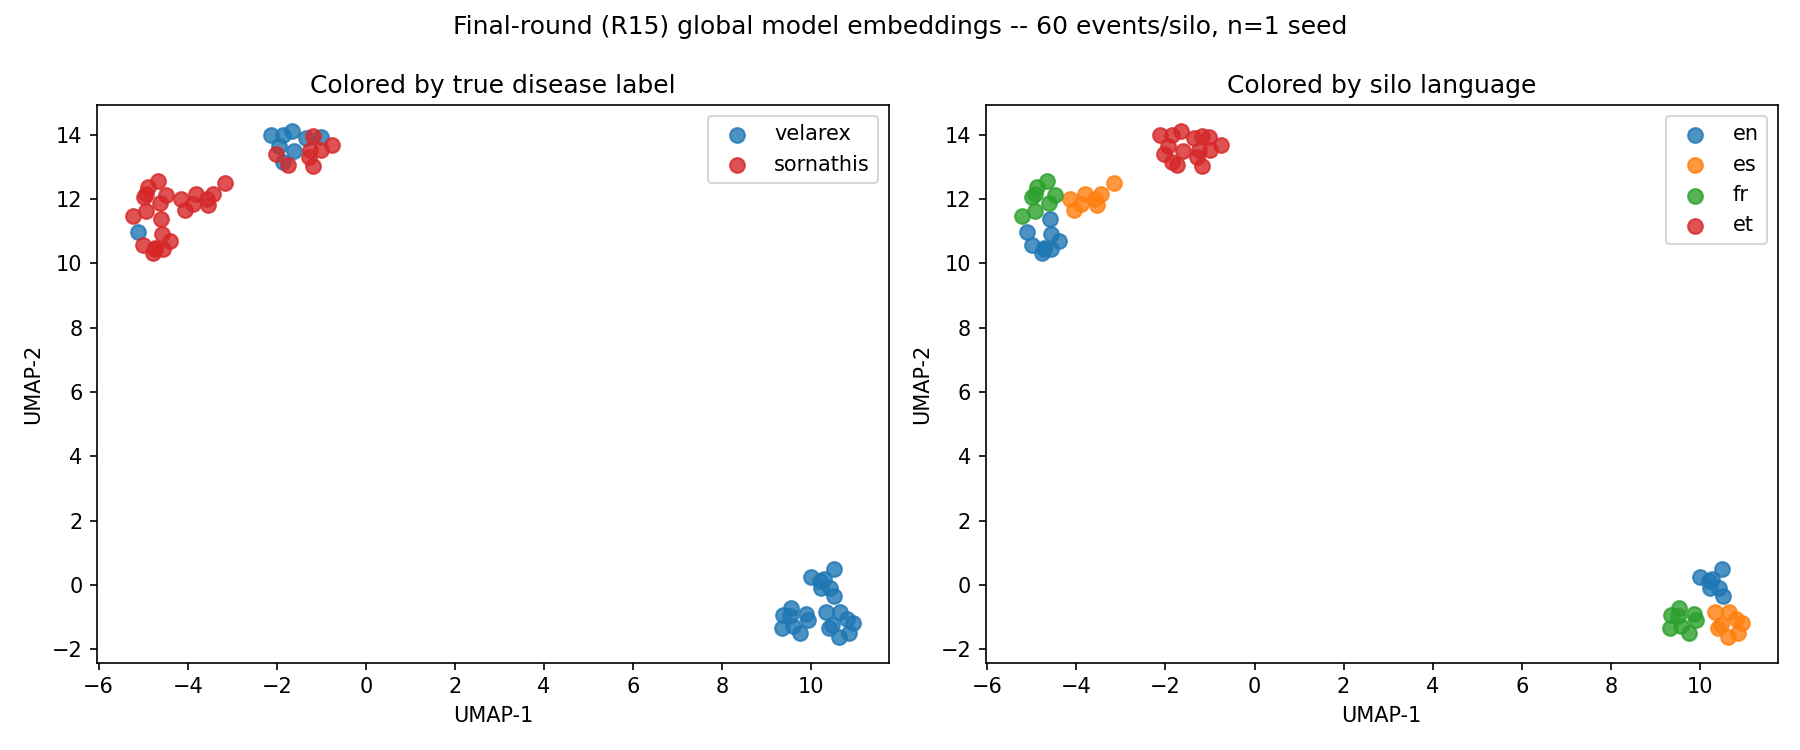
\includegraphics[width=0.95\textwidth]{bonus_fig3_multilingual_global_clusters.png}
  \caption{Final-round (R15) global-model probe embeddings (UMAP), four-silo
  run (en/es/fr/et), colored by true disease label (left) and by silo
  language (right).}
  \label{fig:bonus-global-clusters}
\end{figure}

Figures~\ref{fig:bonus-unknown-disease-rotation-enesfr}
and~\ref{fig:bonus-unknown-disease-rotation-enesz} examine novel-disease
(Morven) detectability as a function of which silo's language receives the
injected cases. Each panel within a figure corresponds to a different
injection language; the Morven-vs-known silhouette is tracked over FL
rounds, broken out by probe language.

\begin{figure}[ht]
  \centering
  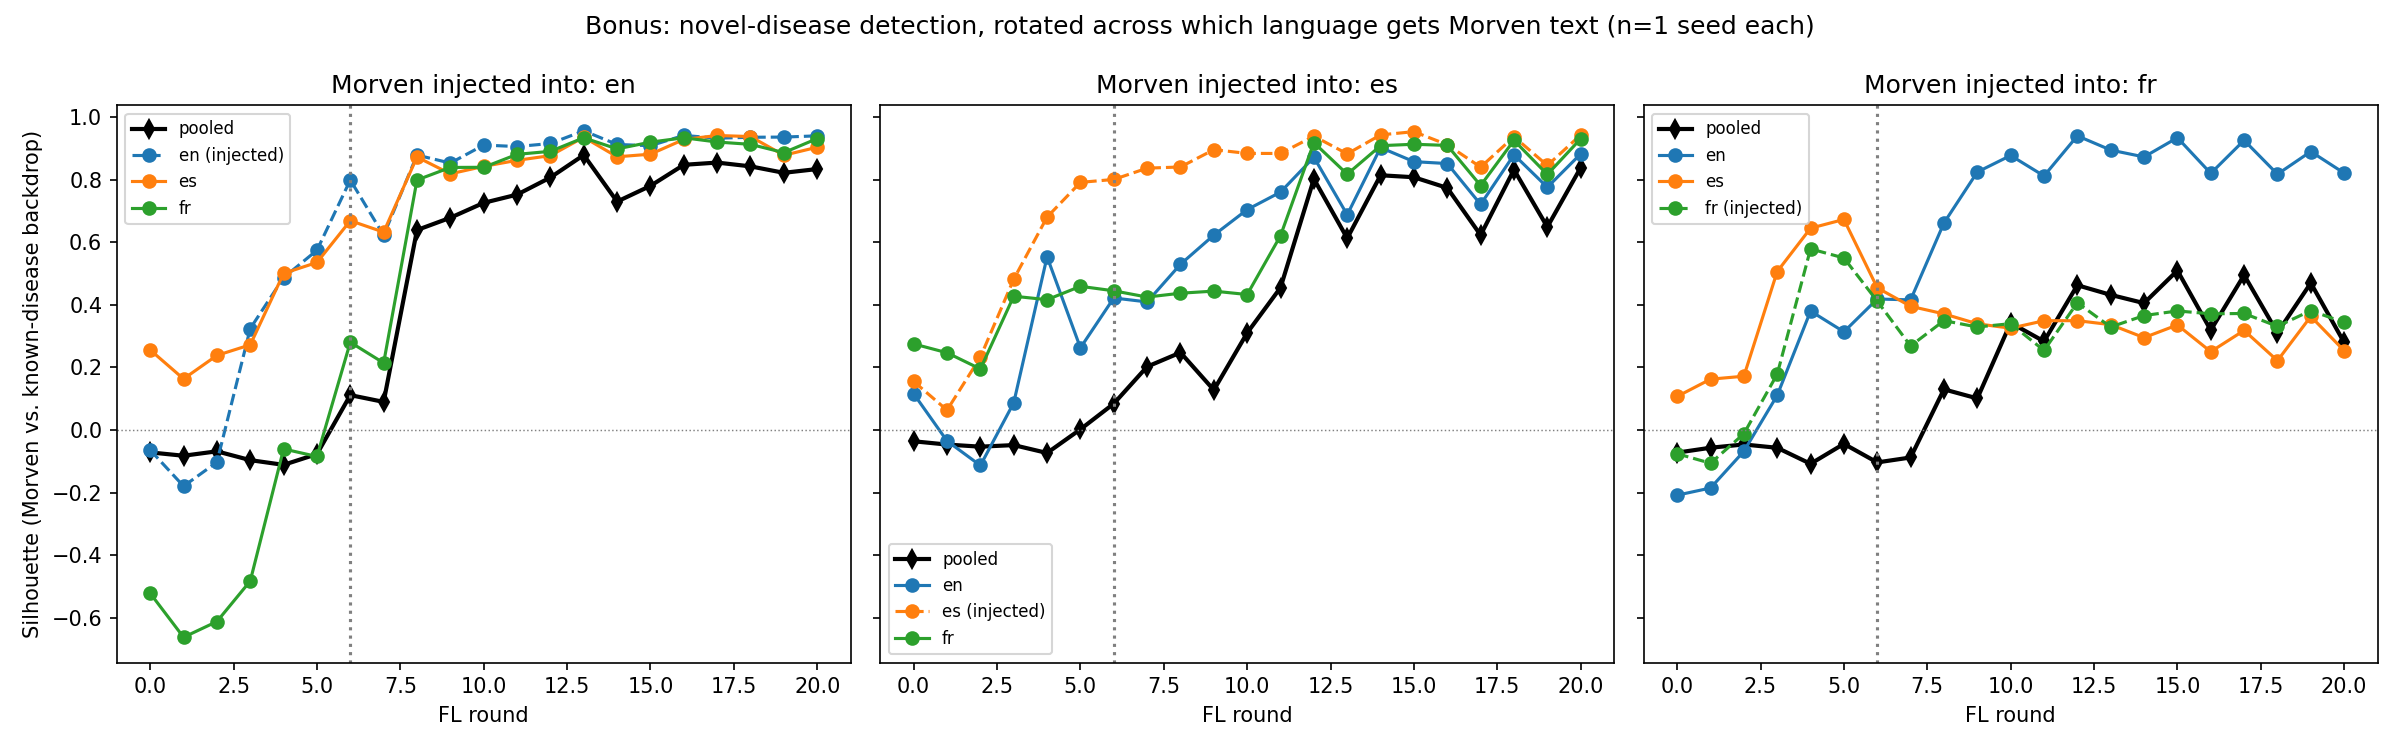
\includegraphics[width=0.95\textwidth]{bonus_fig5_unknown_disease_rotation_enesfr.png}
  \caption{Novel-disease (Morven) injection experiment, English/Spanish/French
  silos: Morven-vs-known silhouette over FL rounds (pooled and per probe
  language), rotated across which silo's language receives the injected
  Morven text (one panel per injection condition). Vertical dotted line marks
  the injection round.}
  \label{fig:bonus-unknown-disease-rotation-enesfr}
\end{figure}

\begin{table}[ht]
  \centering
  \caption{Final-round (R20) Morven-vs-known silhouette, by probe language,
  English/Spanish/French rotation, $n=1$ seed per injection condition.}
  \begin{tabular}{lrrrr}
    \toprule
    Injected into & en & es & fr & Pooled \\
    \midrule
    en & 0.940 & 0.904 & 0.931 & 0.834 \\
    es & 0.882 & 0.943 & 0.931 & 0.838 \\
    fr & 0.821 & 0.254 & 0.344 & 0.280 \\
    \bottomrule
  \end{tabular}
  \label{tab:bonus-unknown-disease-enesfr}
\end{table}

The en/es/zh rotation (Figure~\ref{fig:bonus-unknown-disease-rotation-enesz},
Table~\ref{tab:bonus-unknown-disease-enesz}) replicates the protocol with
Chinese in place of French, allowing the French-injection anomaly to be
assessed against an independent third language.

\begin{figure}[ht]
  \centering
  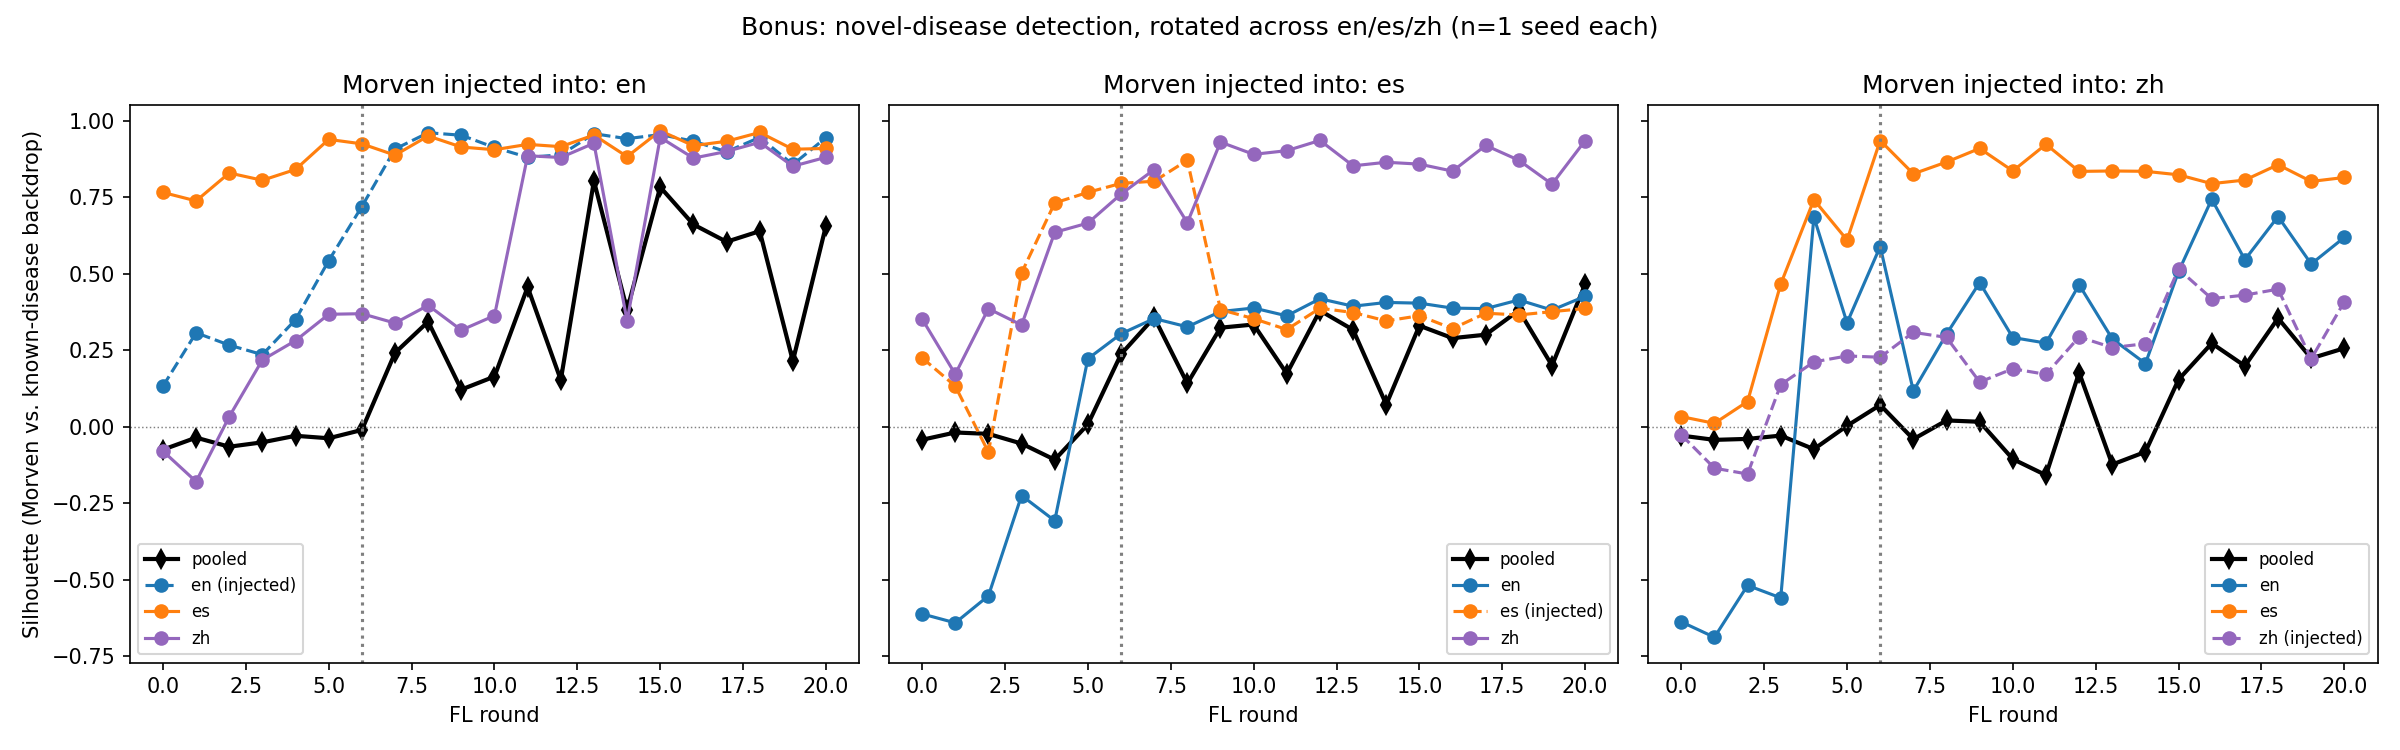
\includegraphics[width=0.95\textwidth]{bonus_fig6_unknown_disease_rotation_enesz.png}
  \caption{Same protocol as Figure~\ref{fig:bonus-unknown-disease-rotation-enesfr},
  English/Spanish/Chinese silos in place of English/Spanish/French.}
  \label{fig:bonus-unknown-disease-rotation-enesz}
\end{figure}

\begin{table}[ht]
  \centering
  \caption{Final-round (R20) Morven-vs-known silhouette, by probe language,
  English/Spanish/Chinese rotation, $n=1$ seed per injection condition.}
  \begin{tabular}{lrrrr}
    \toprule
    Injected into & en & es & zh & Pooled \\
    \midrule
    en & 0.945 & 0.910 & 0.881 & 0.658 \\
    es & 0.427 & 0.387 & 0.936 & 0.467 \\
    zh & 0.619 & 0.815 & 0.409 & 0.257 \\
    \bottomrule
  \end{tabular}
  \label{tab:bonus-unknown-disease-enesz}
\end{table}

Notably, in both the en/es/fr and en/es/zh rotations, injecting Morven via
French or Chinese yields markedly lower pooled and cross-language
silhouette ($0.280$ and $0.257$ respectively) than injecting via English
or Spanish in the same rotation. This is a single seed per condition, but
the pattern repeats across two unrelated rotations sharing no common
second language: worth flagging as a candidate hypothesis (injection
language affects detectability) for follow-up, while being explicit that
$n=1$ per condition means it could also be a shared artifact of how
French/Chinese text is tokenized or embedded by this particular
multilingual backbone. We do not present this as a finding; it is a
candidate hypothesis pending replication.

Figure~\ref{fig:bonus-unknown-disease-clusters-enesz} provides the
corresponding UMAP visualisation for the en/es/zh runs, showing cluster
geometry at the final round for each injection condition.

\begin{figure}[ht]
  \centering
  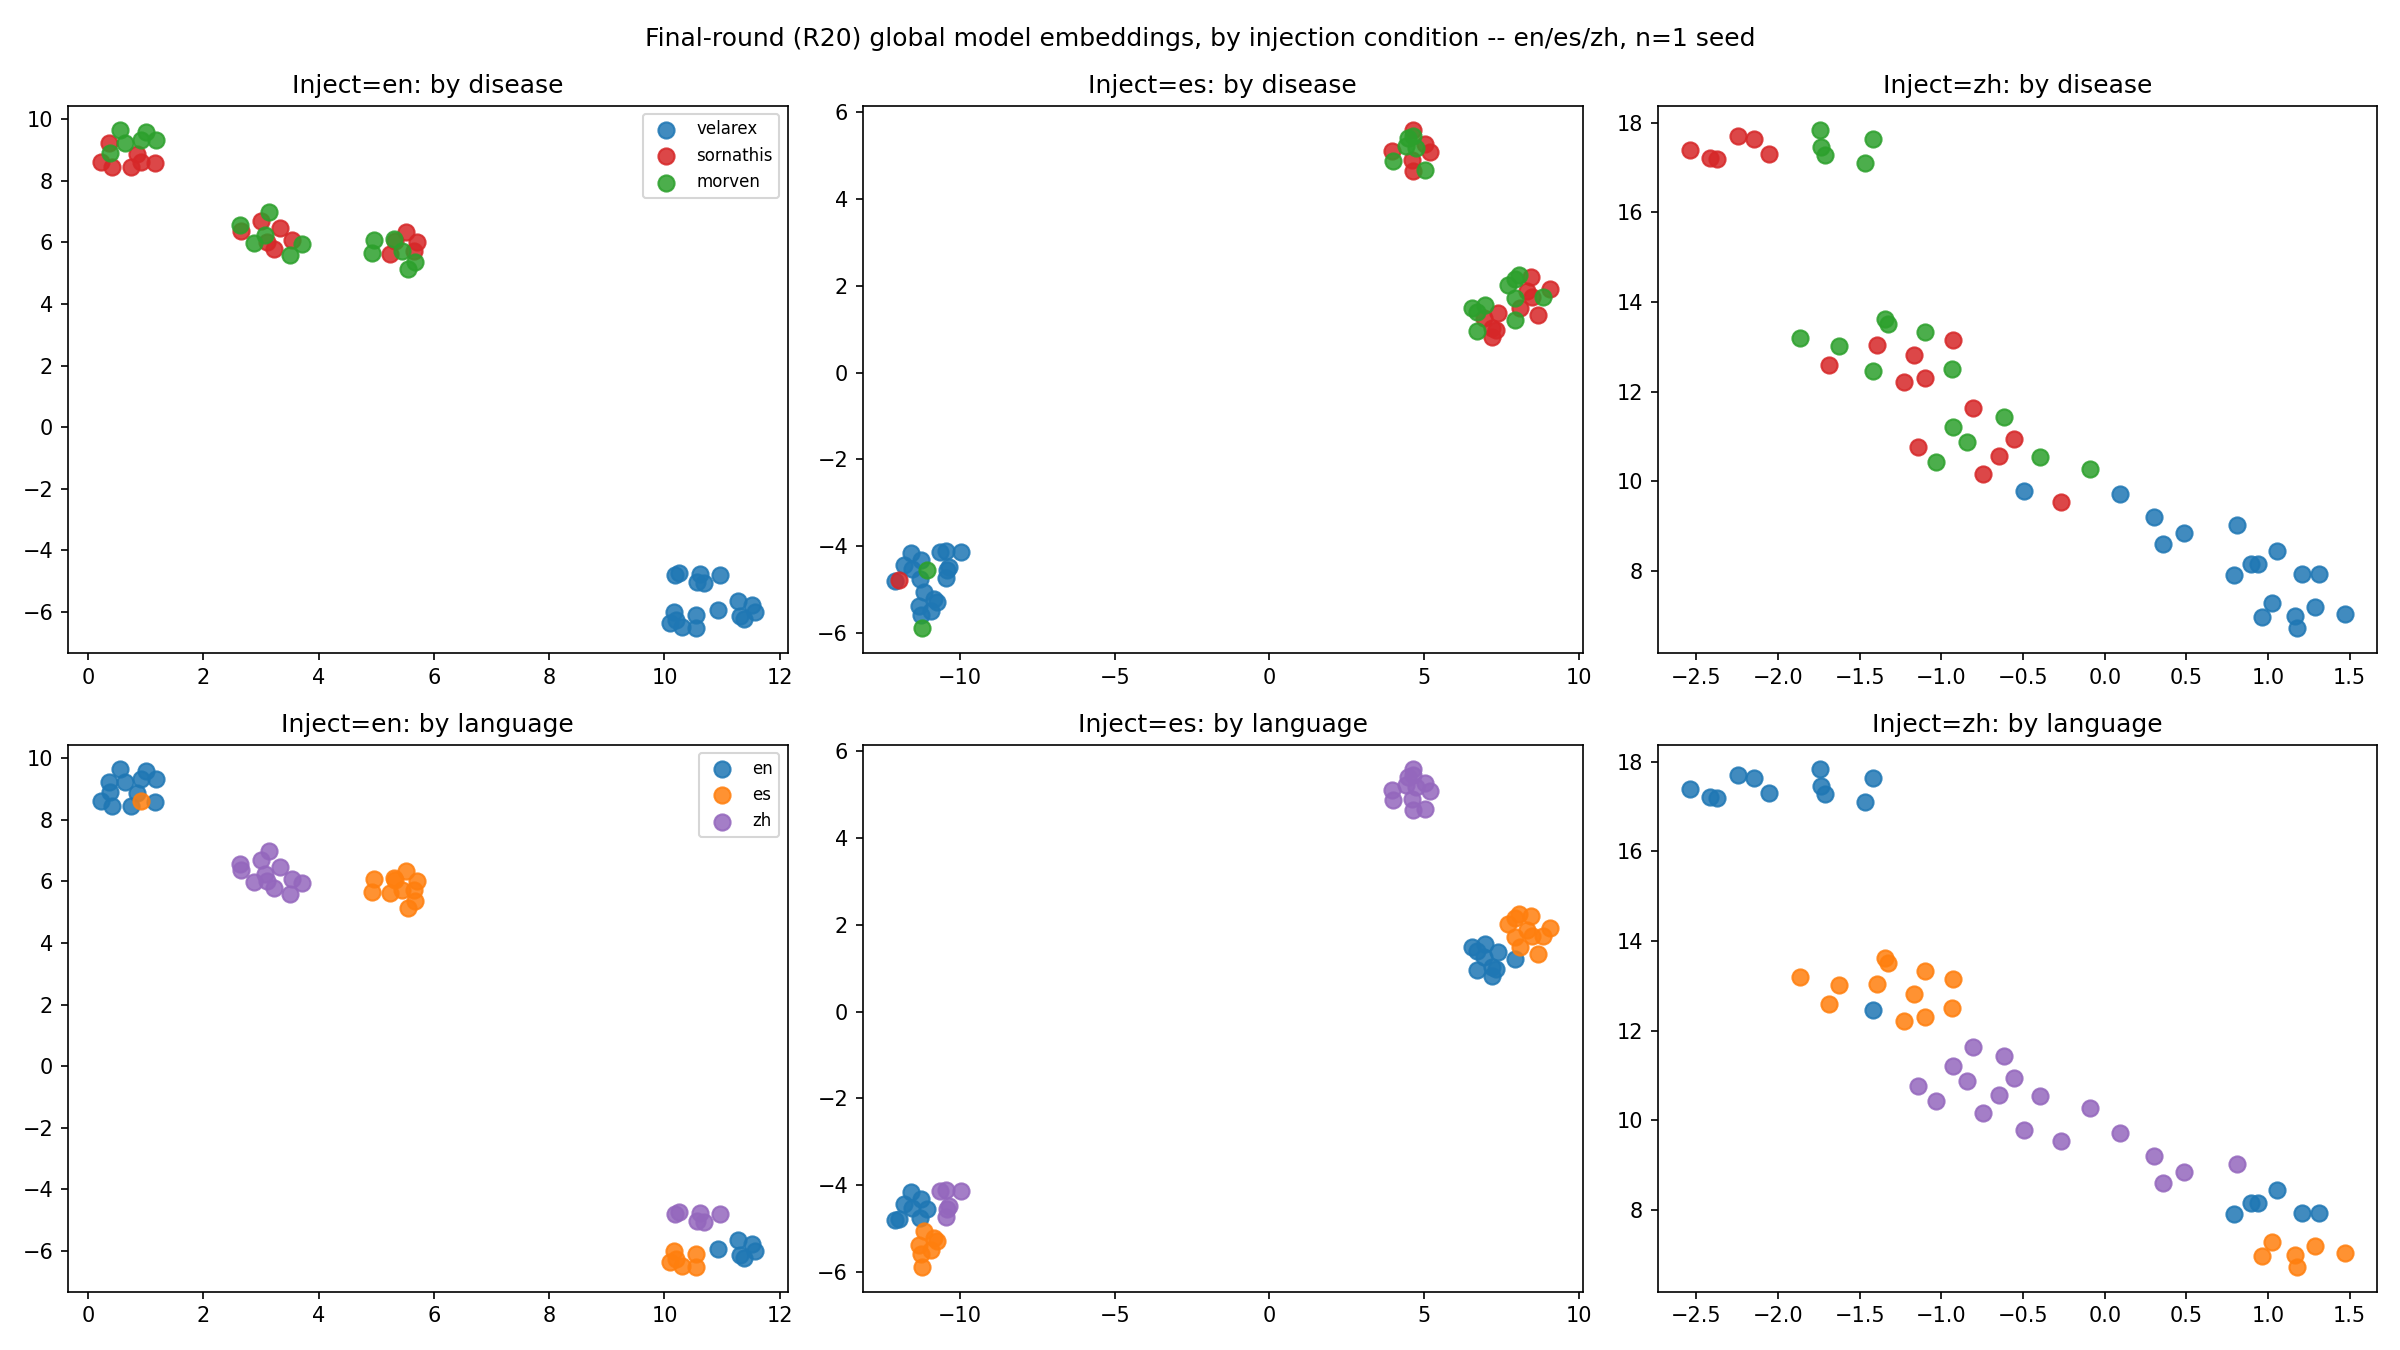
\includegraphics[width=0.95\textwidth]{bonus_fig7_unknown_disease_clusters_enesz.png}
  \caption{Final-round (R20) global-model probe embeddings (UMAP),
  English/Spanish/Chinese rotation: top row colored by disease (Velarex,
  Sornathis, Morven), bottom row colored by probe language, one column per
  injection condition.}
  \label{fig:bonus-unknown-disease-clusters-enesz}
\end{figure}


\end{document}
